\documentclass[gchron, manuscript]{copernicus}

% copernicus.cls loads `supertabular` natively but NOT `longtable`.
% chapter1_body.tex's apatite step-heat table (\chplandscape-wrapped,
% a no-op here) now uses `longtable` instead of `supertabular` -- see
% the comment at that table in chapter1_body.tex for why. Load it
% explicitly so \begin{longtable} is defined in this standalone
% manuscript too (dissertation_preamble.tex already loads it for the
% thesis side).
\usepackage{longtable}

\begin{document}

\title{A Simple Method for Helium Step Heat Experiments at High Water or Sulfur Fugacity}

\Author[1][bthyer@caltech.edu]{Ben J.}{Thyer}
\Author[1]{Jonathan}{Treffkorn}
\Author[1]{Ken A.}{Farley}

\affil[1]{Division of Geological and Planetary Sciences, California Institute of Technology, Pasadena, CA 91125, USA}

\runningtitle{Helium Step Heat Experiments at High Water or Sulfur Fugacity}

\runningauthor{Thyer et al.}

\received{}
\pubdiscuss{}
\revised{}
\accepted{}
\published{}

\firstpage{1}

\graphicspath{{../Figures/source/}{../Figures/generated/}}

\maketitle

\begin{abstract}
% =============================================================
%  chapter1_abstract.tex
%  Shared abstract text for Chapter 1 / TubeMethodPaper.tex.
%
%  Kept separate from the surrounding \begin{abstract}...\end{abstract}
%  wrapper because that environment is NOT class-agnostic: under
%  copernicus.cls it renders in place as the paper's abstract, but
%  under caltech_thesis.cls the `abstract` environment is redefined
%  to break out into a new unnumbered "Abstract" chapter (via
%  \extrachapter), which is only appropriate once, at the front of
%  the whole dissertation (see dissertation.tex's own Abstract
%  chapter) -- not again in the middle of Chapter 1. So each wrapper
%  supplies its own environment/heading around this same raw text.
%
%  Edit this file (not TubeMethodPaper.tex or chapter1.tex directly)
%  to keep the journal paper and the dissertation chapter in sync.
% =============================================================
Helium isotope studies and U-Th/He geochronology of sulfur-bearing and hydrous minerals offer direct windows into the timing and context of hydrothermal mineralization, provided the conditions governing radiogenic helium retention and loss in nature are known. However, assessing helium retentivity at elevated temperatures is currently hampered by these minerals\textquotesingle{} instability under the high-temperature, high-vacuum conditions of conventional helium step-heating experiments. This paper introduces a novel method for conducting helium step-heating experiments under hydrothermal and sulfur-saturated conditions, designed to extend our knowledge of helium diffusion kinetics in hydrous and sulfur-bearing mineral phases. In this approach, silica glass ampoules encapsulate the mineral of interest, maintaining internally sulfur- or water vapor-saturated conditions against the ultra-high vacuum of the surrounding extraction line, while the high helium permeability of fused silica permits quantification of evolved helium using standard temperature control and mass spectrometry procedures. This work presents the experimental framework and key equations necessary to deconvolve the processes of helium permeation through the silica ampoule from the thermally activated degassing of helium from the encapsulated mineral. Permeation lag is quantified with a first-order permeation model and removed by one of two routes: the \emph{permeation step method}, which measures the ampoule's residual helium directly with low-temperature permeation steps, or, where those yields fall to blank level, the \emph{bounding method}, which constrains that residual from above by assuming steady-state permeation during long steps. Both rest on the ampoule's permeation rate constant, which is measured during the experiment itself rather than taken from the literature. Validation experiments measuring helium permeation through empty ampoules and ampoules containing only water, sulfur, or Durango apatite demonstrate that permeation lag is readily correctable in well-designed experiments and characterize the extent to which water and sulfur influence the helium permeability of fused silica. While sulfur-saturated experiments are straightforward to carry out with this method, several tractable complications are identified for experiments when significant water is present. This method expands standard experimental capabilities to encompass mineral phases that decompose under high vacuum, including sulfides and iron oxyhydroxides, opening new avenues for thermochronometric investigation of hydrothermal systems.

\end{abstract}

%% ---------------------------------------------------------------
%% NOTE: Geochronology does not typeset a separate "Plain Language
%% Summary" section in the manuscript PDF. Copernicus instead asks
%% for a short, non-technical "short summary" pasted directly into
%% the online submission form. The text below is kept here (as a
%% comment, so it does not print) purely so it can be
%% copied into the submission form's short-summary field.
%%
%% U-Th/He Thermochronology is a technique geochemists use to understand a region's thermal history. This approach could potentially be applied to minerals that form in hydrothermal systems, such as sulfide ore minerals and iron oxides, to directly date events like ore deposit formation or ancient fluid circulation; however, it requires knowledge of how helium is lost within the mineral at elevated temperatures. Unfortunately, the measurements necessary to study this process are difficult because these minerals decompose when heated in the strong vacuum of the experimental environment, producing results that do not mimic natural conditions.
%% 
%% This paper describes a new experimental technique to address this problem. The mineral sample is sealed inside a small silica glass tube, which keeps the mineral surrounded by water vapor or sulfur gas, providing the conditions it needs to stay stable, even while the outside of the tube is under high vacuum. Silica glass is naturally permeable to helium, so helium released from the mineral as it is heated can still pass through the tube walls and be detected by standard instruments. The key analytical challenge is separating the helium signal coming from the mineral itself from the delay introduced by helium slowly diffusing through the glass tube walls. This chapter presents the equations and experimental procedures needed to make that separation and tests the approach using simple calibration experiments. The results show the method works well for sulfur-saturated experiments but also reveal some manageable complications for water-saturated experiments. This technique extends helium-based age-dating methods to a new class of geologically important minerals.
%% ---------------------------------------------------------------

% chapter1_body.tex wraps its widest tables in \chplandscape so the
% dissertation version (Chapter1/chapter1.tex) can rotate them to
% landscape for extra width while this journal manuscript keeps them
% portrait at their original compact size -- defined here as a no-op.
\newenvironment{chplandscape}{}{}

% =============================================================
%  chapter1_body.tex
%  Shared, class-agnostic body of Chapter 1 / TubeMethodPaper.tex
%  (Introduction through Conclusions -- everything between the
%  abstract and the end-matter/bibliography).
%
%  \input{} by BOTH:
%    - Chapter1/Writing/TubeMethodPaper.tex   (Copernicus journal paper)
%    - Chapter1/chapter1.tex                (dissertation chapter, caltech_thesis)
%  so the scientific content never has to be maintained in two places.
%  Edit this file, not the two wrappers, for any content change.
%
%  Portability notes:
%   - \introduction / \conclusions (Copernicus shorthands for
%     \section{Introduction} / \section{Conclusions}) have been
%     expanded to plain \section{} calls below so this file has no
%     dependency on copernicus.cls.
%   - Tables use \tophline/\middlehline/\bottomhline (Copernicus's
%     names for booktabs' \toprule/\midrule/\bottomrule). The
%     \providecommand block just below defines them as booktabs
%     aliases ONLY if not already provided by the wrapping class
%     (copernicus.cls defines its own, so this is a no-op there).
%     Whichever wrapper does NOT already provide them must load the
%     `booktabs` package itself (dissertation_preamble.tex already does).
%   - The multi-page apatite step-heat table uses `longtable`, not
%     `supertabular` (switched from supertabular -- see the comment at
%     that table below for why). copernicus.cls does NOT load
%     `longtable` natively, unlike `supertabular`, so TubeMethodPaper.tex
%     loads it explicitly; the thesis side gets it from
%     dissertation_preamble.tex. The SI's other multi-page tables still
%     use `supertabular` (portrait) or `longtable` (the three
%     \chplandscape-wrapped ones) -- see chapter1_SI_body.tex.
%   - Cross-references to the SI (e.g. "supplementary Fig.~\ref{...}",
%     "supplementary Eq.~\eqref{...}") use real \ref{}/\eqref{} against
%     labels defined in chapter1_SI_body.tex. These resolve correctly in
%     the dissertation, where chapter1.tex and chapter1_SI.tex are both
%     \input{} into the same dissertation.tex document (shared .aux).
%     They will render as "??" in the standalone TubeMethodPaper.tex/
%     SI.tex compile, since those are two separate documents and
%     \ref{}/\eqref{} cannot resolve across them -- to be addressed
%     separately (e.g. reverting to manual "supplementary Fig. N" text,
%     or a cross-document referencing package) when preparing that
%     standalone submission.
% =============================================================
\providecommand{\tophline}{\toprule}
\providecommand{\middlehline}{\midrule}
\providecommand{\bottomhline}{\bottomrule}

\section{Introduction}

Noble gas geochronology and thermochronometry (\textsuperscript{40}Ar/\textsuperscript{39}Ar and U-Th/He) on hydrous and sulfur-bearing mineral phases such as hornblende, clay minerals, biotite, goethite, and pyrite have already been leveraged as a powerful tool for understanding regional thermal histories as well as the timing of iron or rare metal mineralization \citep{mcinnes2005,heim2006,vasconcelos2013,nomade2004,yakubovich2020,yakubovich2021}. The interpretation of these data, however, is often complicated by the fact that helium (or argon) within hydrous or sulfur-bearing phases often degasses differently in the laboratory and in nature \citep{hanson1975,lee1993,lo2000,farley2024}.

Experiments aiming to characterize the migration mechanisms and rates of noble gasses through hydrous phases yield different results when conducted under hydrothermal conditions as opposed to traditional experimental methods in vacuo. Hydrothermal step heat experiments for argon in biotite and hornblende showed higher retentivity and comparatively favored diffusive loss mechanisms relative to experiments conducted in vacuo, and these results are more likely to accurately reflect loss mechanisms in nature \citep{harrison1982,harrison1985}; however, such experiments are labor-intensive and comparatively inflexible relative to modern helium step heat methods \citep{farley1999}.

Recently, some workers have taken advantage of the high helium permeability and selectivity of pure silica glass when designing novel experimental methods for U-Th/He geochronology \citep{yakubovich2020,yakubovich2021}, but these ideas have only been applied in a limited way to characterize helium migration in sulfur-bearing or hydrous phases (e.g., monotonic ramped heating experiments: \citealp{yakubovich2019}). This work aims to apply decades of research on helium permeability, solubility, and diffusion in fused silica glass \citep[e.g.,][]{jones1953,norton1953,rogers1954,altemose1961,swets1961,doremus1966,masaryk1968,shelby1971,shelby1972,shelby1976,shackelford1972} to adapt existing agile step-heat methods \citep{farley1999} to investigate helium loss rates and mechanisms in sulfur-bearing and hydrous mineral phases. 

Encapsulating minerals in silica glass ampoules allows experimentalists to maintain hydrothermal or sulfur-saturated conditions within the ampoule without otherwise altering the experimental design. Depending on the thermodynamics of the phase of interest, this method may stabilize the phase at elevated experimental temperatures, allowing for detailed characterization of helium migration in sulfide and hydrous minerals that hitherto has remained poorly understood (Fig.~\ref{fig:mineral-grid}).

\begin{figure}[htbp]
\centering
% \renewcommand{\arraystretch}{1.3}
% \rotatebox{90}{...} (no options) rotates around the box's bottom-left
% corner, not its center -- next to a row of images much taller than the
% label text, that left "Pyrite" visibly anchored toward the bottom of its
% row while "Arsenopyrite" (long enough to nearly fill the row on its own)
% looked centered mostly by coincidence. \rotatebox[origin=c]{90}{...}
% rotates around the text's own center instead, which centers both labels
% against their image row regardless of word length.
\setlength{\tabcolsep}{4pt}
\begin{tabular}{cccc}
 & \textbf{Control} & \textbf{Buffered} & \textbf{Unbuffered} \\[2pt]

\rotatebox{90}{\textbf{Pyrite}} &
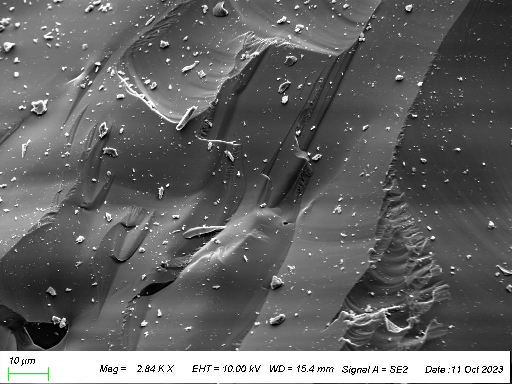
\includegraphics[width=0.28\textwidth]{LVPY_control_10um0.pdf} &
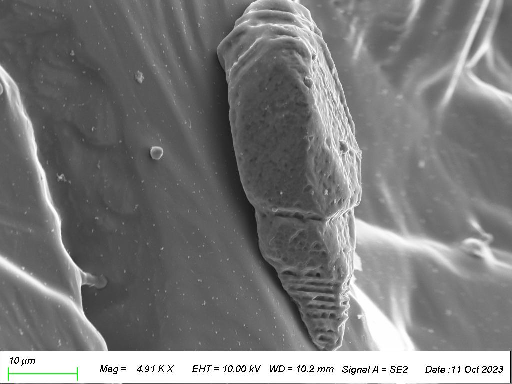
\includegraphics[width=0.28\textwidth]{LVPy_buff_600_8Hr_10um07.pdf} &
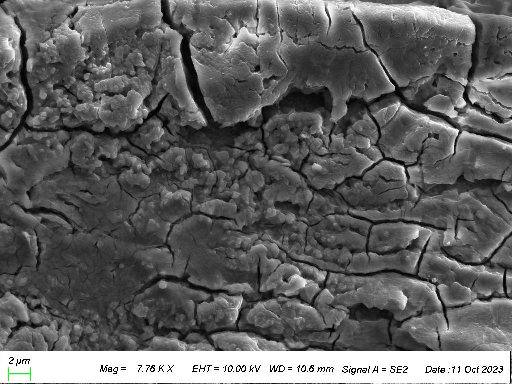
\includegraphics[width=0.28\textwidth]{LVPy_open_400_5Hr_2um11.pdf} \\[4pt]

\rotatebox{90}{\textbf{Arsenopyrite}} &
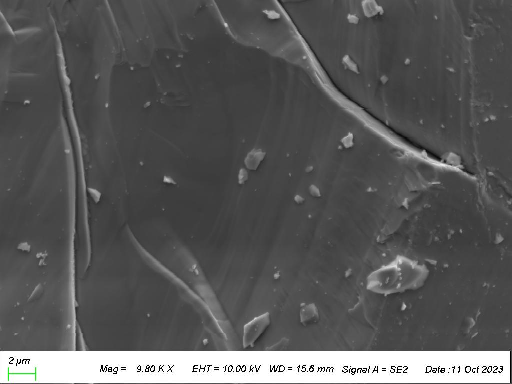
\includegraphics[width=0.28\textwidth]{Asp_control_2um7.pdf} &
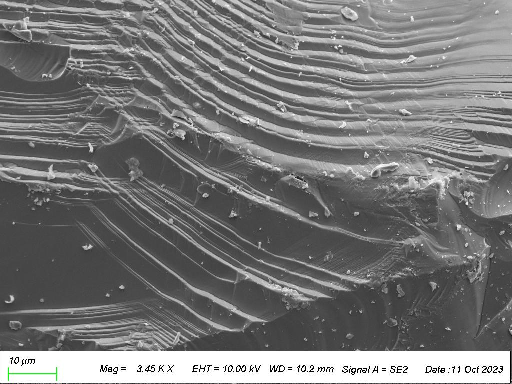
\includegraphics[width=0.28\textwidth]{asp_buff_400_8Hr_10um12.pdf} &
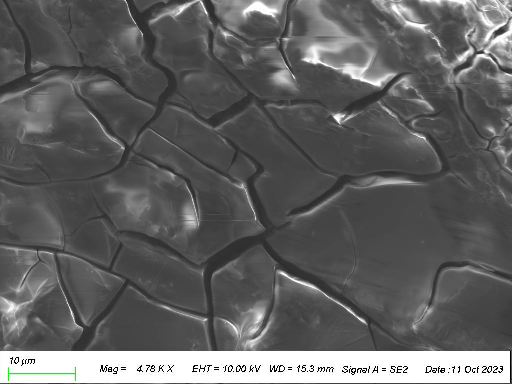
\includegraphics[width=0.28\textwidth]{Asp_bigClosed_400C_4hr_10um5.pdf} \\

\end{tabular}
\caption{Secondary electron SEM images of pyrite (top row) and arsenopyrite (bottom row) surface textures before heat treatment (control), and after heat treatment at 400°C for at least 4 hours, both unbuffered and buffered in a silica glass ampoule with fused sulfur or mineral realgar (AsS) for pyrite and arsenopyrite respectively. The buffered samples maintain the smooth surfaces and clear cleavage faces that the controls have, showing no evidence of decomposition. The unbuffered samples show clear evidence of decomposition by devolatilization, indicated by the formation of contraction cracks and surface roughening. Using silica glass ampoules to buffer samples within controlled microenvironments can prevent phase decomposition at the elevated experimental temperatures typical of helium step heat experiments. See the supplement \S\ref{sem-imaging-of-buffered-and-decomposed-sulfides} for details on the experimental methods and sample preparation.}
\label{fig:mineral-grid}
\end{figure}

\section{Experimental Methods}\label{experimental-methods}

\begin{figure}[t]
\centering
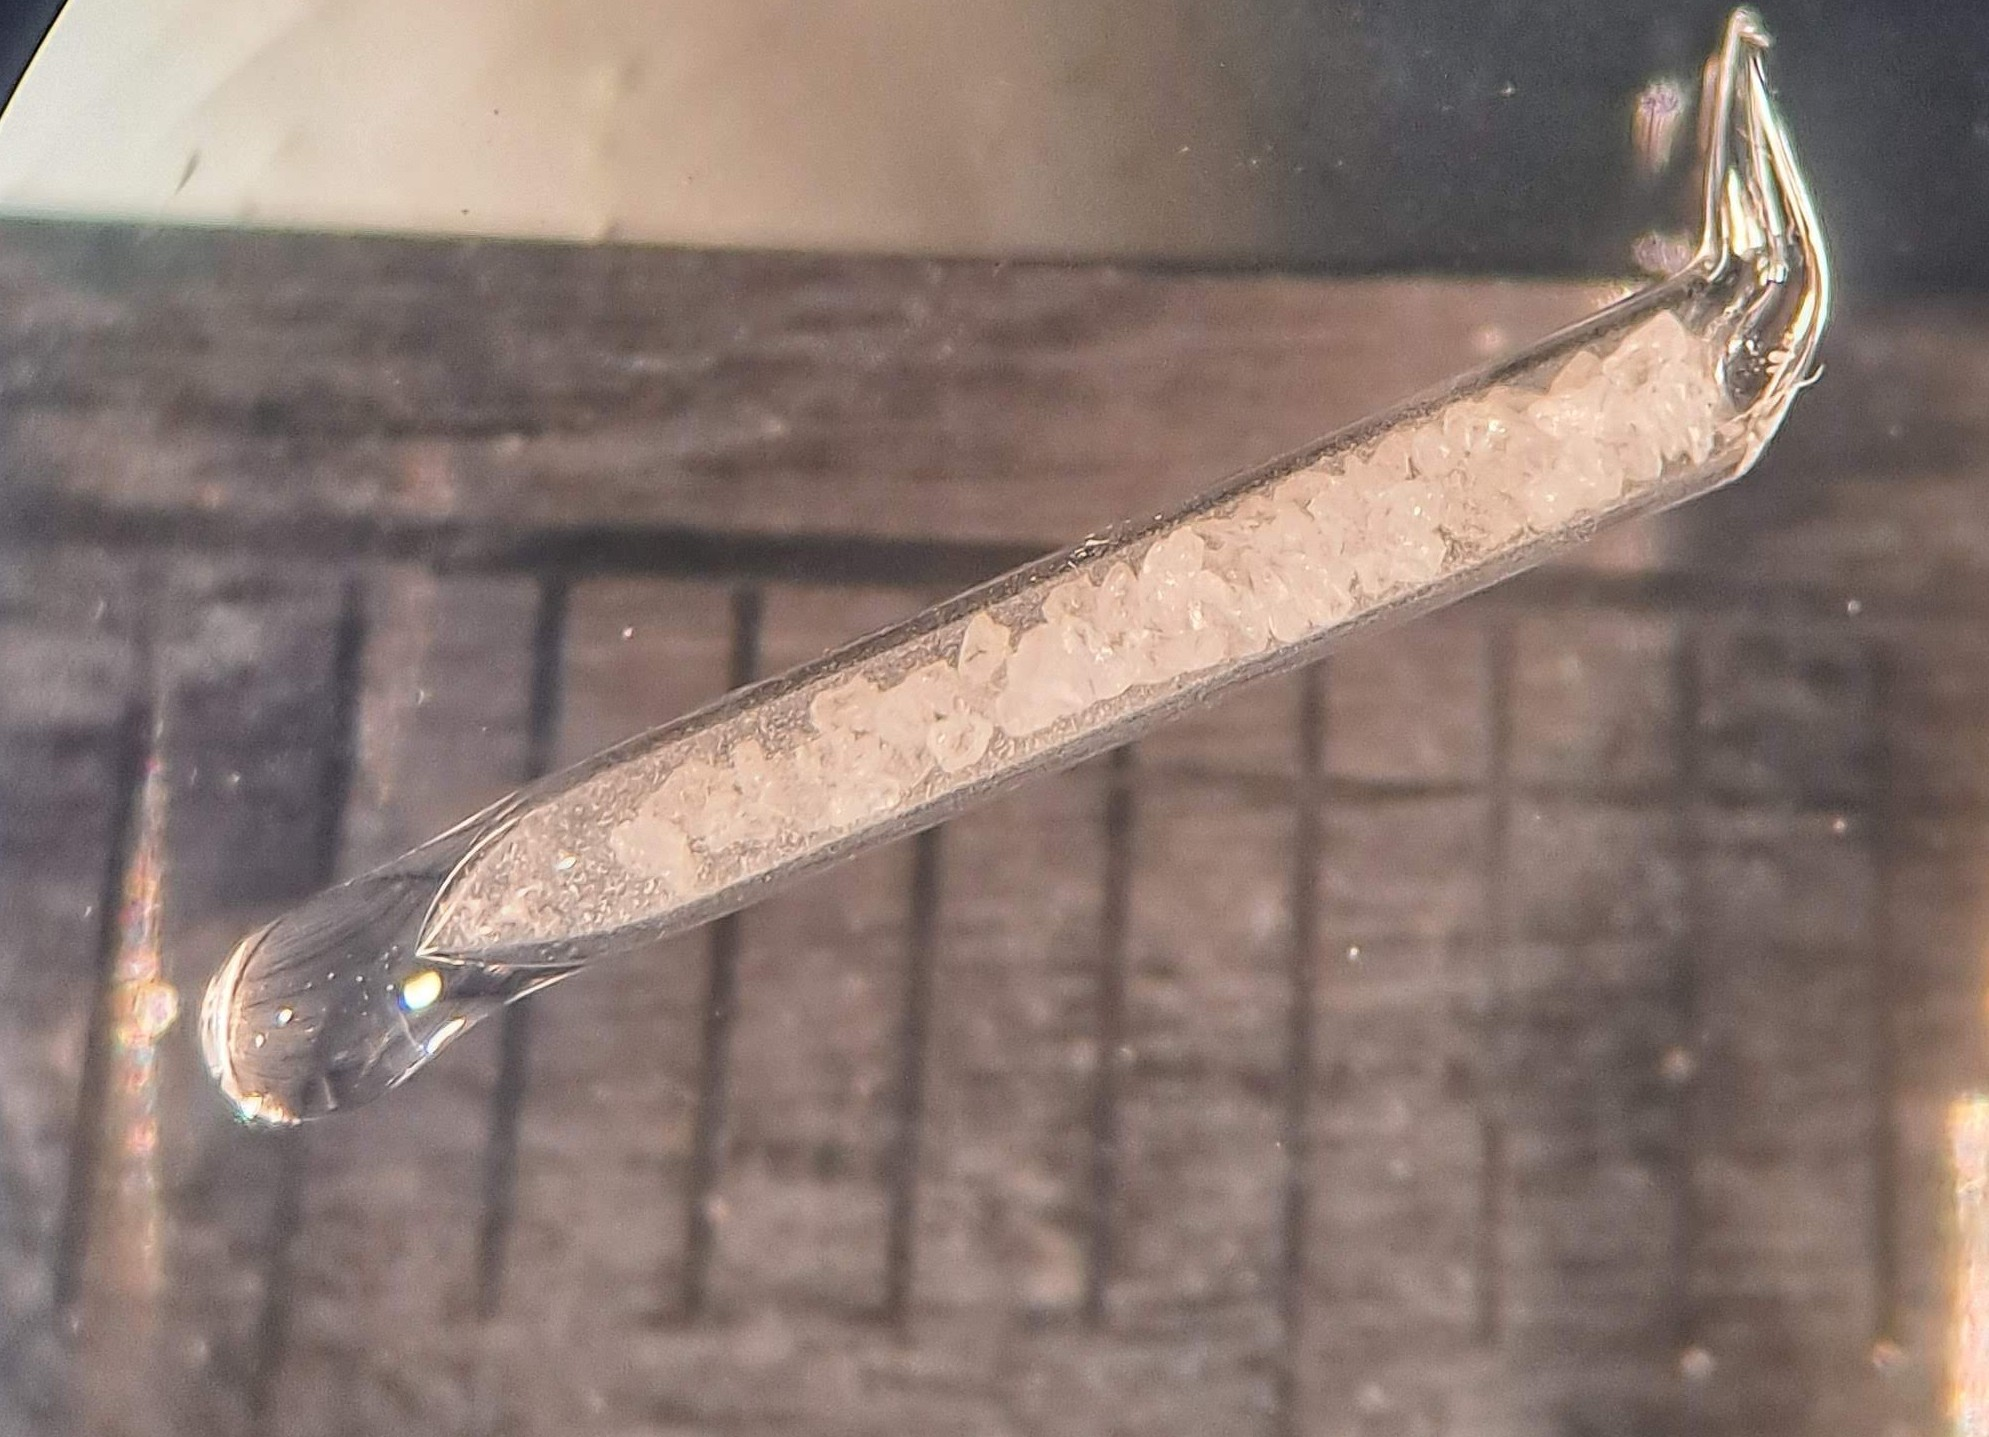
\includegraphics[width=8.3cm]{Apatite_tube.jpg}
\caption{A typical silica glass ampoule used for helium step heat experiments. The ampoule shown here contains Durango Apatite crushate sieved to 300 µm (radii $\approx$ 150 µm). The ampoule is roughly one cm long and one mm wide. The bars visible in the background are each separated by 1 mm.}
\label{fig:ampoule-photo}
\end{figure}

Five helium step heat experiments of sealed silica glass ampoules were undertaken at Caltech to demonstrate the applicability of equations derived here to real helium step heat experiments of geologic materials using a projector-lamp heating apparatus, described in detail in \citet{farley1999}. Four of these experiments involved introducing helium into empty, water-filled, and sulfur-filled ampoules, then measuring helium permeation to assess the applicability of theory outlined in this chapter to helium step heat experiments at Caltech, and to reproduce measurements of permeability rates from the literature \citep{norton1953,jones1953,swets1961,altemose1961}. The fifth experiment was a standard helium step heat experiment on encapsulated Durango apatite, a widely used standard for helium diffusion experiments and U-Th/He thermochronometry \citep{zeitler1987,wolf1996,farley2000,shuster2005,shuster2006,flowers2007}. The aim of that experiment was to be a practical test in deconvolving the process of helium permeation through silica glass ampoules from thermal helium loss of a well-studied geologic material. Table~\ref{tab:ampoule-dimensions} summarizes the dimensions, geometric factors, and encapsulated materials of this work.

% Fixed-width p{...} columns (13.6cm) don't shrink with font size alone --
% wrapped in \resizebox to hard-guarantee it fits the 5.5in Caltech text
% width. Safe here because this is a single-page `table`/`tabular` (not
% longtable/supertabular, which cannot be resizebox-wrapped). Kept in
% portrait (no \chplandscape) at the default \AtBeginEnvironment{table}{
% ...\footnotesize} size -- same treatment as the other tables -- per
% feedback that this table read oddly enlarged/landscaped relative to the
% rest and fit fine in portrait before.
\begin{table}[t]
\centering
\caption{Silica Glass tubes that were the subject of helium step heat experiments in this work. Ampoules labeled ``Quad'' had evolved 4He quantified by isotope dilution using a Pfeiffer Prisma QMS 200 quadrupole mass spectrometer, whereas ampoule labeled ``MC'' had both evolved 3He and 4He quantified using a Helix-MC-Plus\textsuperscript{10K} multi-collector mass spectrometer. Where 3He was measured, the ampoule was soaked in tank helium with an isotope ratio of \textasciitilde0.15 Ra}
\label{tab:ampoule-dimensions}
\resizebox{\textwidth}{!}{%
\begin{tabular}{p{1.8cm}p{1.4cm}p{1.8cm}p{1.8cm}p{1.8cm}p{1.2cm}p{1.8cm}p{2.2cm}}
\tophline
Ampoule Contents & Mass Spec. & Inner \newline Diameter \newline µm & Outer \newline Diameter \newline µm & Geometric factor \emph{G} \newline cm\textsuperscript{-2} & Volume Ratio $\left(\frac{V_{glass}}{V_{gas}}\right)$ & Content \newline Mass & Helium \newline Source \\
\middlehline
Empty & Quad & 630 & 960 & 4785.3  & 1.32 & --- & Atmosphere \\
Empty & MC & 747 & 1159 & 3263.9 & 1.41 & --- & Tank He \\
Sulfur & MC & 529--550 & 835--872 & 5992.1 & ~1.5 & \textasciitilde0.2 mg & Tank He \\
Water & MC & 487--515 & 734--776 & 7789 & 1.27 & \textasciitilde0.5 mg  & Tank He \\
Durango \newline Apatite & Quad & 850 & 1350 & 2393.5 & 1.52 & 3.18 mg & Radiogenic \\
\bottomhline
\end{tabular}%
}
\end{table}

To prepare the silica glass ampoules, \textasciitilde10 cm long segments of pure silica glass tubes with an outer diameter of 4 mm and an inner diameter of 3 mm were submerged and sonicated within acetone, ethanol, then MilliQ water baths in sequence, and then were dried overnight in a 100°C oven. The glass tubes were hand-pulled into thin pipettes with a jewelry welding torch and their thin ends were fused closed.

After the glass had cooled, degassed lab-grade sulfur, distilled water, or Durango apatite were added to some of the tubes. Two tubes were left empty. To seal, the top of each pipette was interfaced with a vacuum line and was pumped to a pressure of \textless0.1 torr. The encapsulated water tube was flash-frozen in liquid nitrogen and then pumped and sealed in a saltwater ice bath to selectively pump away atmospheric gasses and not water. Sublimation of sulfur and water ice during pumping was minor. The primary motivation for pumping the tube to rough vacuum was to aid the sealing process. After rough vacuum was achieved, a fine-tipped welding torch was used to seal the top of each ampoule. To determine the geometric factors for permeation of the ampoules, the inner and outer diameters of each ampoule were determined using the measurement function of the Amscope stereo microscope software, which was calibrated and tested during early development of this method.

Except for the encapsulated Durango apatite ampoule, helium gas needed to be introduced into the sealed ampoules before they were loaded into the projector lamp heating cells. About 15 nccSTP of atmospheric helium was introduced into the empty ampoule used for the quadrupole mass spectrometer experiment by heating the ampoule in a muffle furnace to \textgreater400°C in atmosphere overnight, which was sufficient to support a short permeation experiment of 4He. However, to conduct step heat permeation experiments on 3He, much larger quantities of helium were necessary. The encapsulated sulfur and water ampoules and the other empty ampoule were soaked in 2-20 torr of high purity tank helium with an isotope ratio of about \textasciitilde0.15 Ra at 300°C for about 24 hours. This procedure introduced 0.6-10 pccSTP 3He and up to 52,000 nccSTP 4He into each tube, allowing for measurements of both 3He and 4He permeation simultaneously.

The sealed ampoules were placed in copper foil packets and mounted to a K-type thermocouple within an ultra-high vacuum projector lamp heating cell described in more detail by \citet{farley1999}. Before each experiment began, each ampoule was washed with ethanol, air-dried, loaded in the lamp cell, pumped to high vacuum, and was held at 100°C for 30 minutes under dynamic vacuum to desorb ethanol, water, and other atmospheric species on the ampoule, copper packet, and lamp cell. Less than 0.5 ‰ of the radiogenic helium in 150µm radius Durango apatite would be expected to degas in 30 minutes at 100°C, which would amount to \textasciitilde0.01 nccSTP for this experiment, using the diffusion parameters of \citet{farley2000} and the forward equations of \citet{fechtigkalbitzer1966}. The atmospheric helium component within the encapsulated Durango Apatite ampoule constrained by permeation steps at the beginning of the experiment was much larger: 1.47 ± 0.18 nccSTP 4He.

We found that the fused silica ampoules were capable of maintaining surprisingly high internal pressures, but ampoules filled with water would often explode at temperatures above 315°C. It is recommended that experimentalists limit the temperature of water-filled ampoules to below 300°C. We have not observed any explosions of sulfur-filled ampoules at any temperature. 

Heating steps and isotopic measurements for all samples were automated using custom LabView routines with the exception of the tank helium-soaked empty tube experiment on the Helix-MC-Plus\textsuperscript{10K} multi-collector mass spectrometer after the 7\textsuperscript{th} measurement. For all other ampoules, a Watlow temperature controller held the ampoule at the temperature set point for a pre-programmed duration, after which the ampoule was allowed to cool while the evolved gas was prepared for measurement for about 25 minutes. After the first 7 measurements, the empty tube experiment on the Helix-MC-Plus\textsuperscript{10K} was instead set to an elevated temperature manually while the evolved gas was allowed to accumulate continuously in an attempt to mitigate uncertainties related to frequently changing temperatures (supplementary Eq.~\eqref{eq:s7-2}; Fig.~\ref{fig:thermal-perturbation-error}) and continued permeation at room temperature during gas cleanup and measurement. The accumulated gas was measured every 40-120 minutes. For this experiment, the temperature was changed either during the 1 minute pump-out of the lamp cell after inletting gas into the mass spectrometer, or a period of helium accumulation for measurement. When the temperature was changed during an accumulation period, no permeability was calculated for that step, and the measured abundances of those steps were used only to track the helium contents of the tube.

Helium isotope measurements of evolved gasses from steps heats of one empty silica glass ampoule and glass-encapsulated sulfur and water ampoules equilibrated with 2-20 torr of high purity tank helium (R $\approx$ 0.15 R\textsubscript{a}) were acquired at Caltech on a Thermo Fisher Helix-MC-Plus\textsuperscript{10K} mass spectrometer in peak hopping mode from November 19\textsuperscript{th}, 2023 to Feburary 15\textsuperscript{th}, 2024. Helium was purified by exposing evolved gasses to a charcoal trap held in liquid nitrogen, a titanium sponge getter, then a SAES NP10 getter before freely expanding into the Helix-MC-Plus\textsuperscript{10K}. 3He was measured with a pulse-counting electron multiplier, while 4He was detected on a Faraday detector. The majority of the analysis time was spent measuring 3He. Every few hours, the background was mass-scanned to set the 3He and 4He measure points; each was taken to be a constant mass offset from the background HD\textsuperscript{+} peak. These mass offsets are precisely measured when tuning the Helix-MC-Plus\textsuperscript{10K} for helium isotope analysis. Months of helium measurements with the Helix-MC-Plus\textsuperscript{10K} at Caltech have shown this approach to be reliable, reproducible, and accurate for helium isotope analysis. Additionally, an electron multiplier monitored atomic mass 3.5 to detect 4He overspray. 4He abundances were very large during these experiments, resulting in a small but measurable 4He overspray of up to 0.68 cps at mass 3.5. These overspray signals at mass 3.5 were always less than 1\% of the 3He signal at mass 3, suggesting that 4He overspray did not significantly affect 3He signals. Measurements of high 3He MM gas standard were analyzed every 8 hours (totaling 116 measurements) to track instrumental drift of 3He and 4He sensitivities and to quantify internal reproducibility. These standards show 3He was internally reproducible to within 5\% (2$\sigma$), whereas 4He was internally reproducible to within 2\% (2$\sigma$), where reproducibility is estimated as the standard deviation divided by the mean.

Helium-4 evolved during step heats of the empty silica glass ampoule equilibrated with atmosphere and the silica glass-encapsulated Durango apatite was quantified using isotope dilution with a high purity 3He spike on a Pfeiffer Prisma QMS 200 quadrupole mass spectrometer from October 30\textsuperscript{th} to November 10\textsuperscript{th}, 2023. Evolved gas from the ampoule in the lamp heating cell was allowed to mix with the 3He spike and the mixture was frozen on charcoal held at 14°K within a cryostat, then helium was selectively released to the mass spectrometer by raising the temperature to 36°K.

A standard gas with a known amount of 4He is routinely measured, at least one time per experiment, to monitor drift in the relative sensitivity of 3He and 4He on the Pfeiffer Prisma QMS 200 quadrupole mass spectrometer. Relative sensitivities are determined for each standard measurement and are linearly interpolated in time for sample measurements. Blanks are approximately 5 pccSTP \textsuperscript{4}He, which is very small compared to all interpreted \textsuperscript{4}He measurements.

\section{Theoretical Framework of Permeation Lag}\label{theoretical-framework-of-permeation-lag}

\begin{figure}[t]
\centering
\includegraphics[width=8.3cm]{Durango_Sim.pdf}
\caption{An illustrative simulation of the effects of permeation lag on step heat measurements of 150 µm radii spheres of Durango apatite encapsulated in a ``standard ampoule'' with an outer diameter of 1mm and inner diameter of 0.6mm, corresponding to a geometric factor \emph{G} of 4350.26 cm\textsuperscript{-2}. Some amount of helium degassed from the apatite during an experimental step remains in the tube during measurement and permeates out in later steps.  The heating schedule of this model system is given in Table~\ref{tab:heating-schedule}. This simple model assumes new temperatures and their corresponding steady-state diffusive concentration profile within the glass ampoule are reached instantaneously. Effects of diffusive disequilibrium, if considered, would change the permeated amount for each step by less than 5\%.}
\label{fig:durango-stepheat-lag-simulation}
\end{figure}

The process of helium permeation through thin walls of an ampoule is rapid but not instantaneous on experimental timescales. Helium evolved from encapsulated minerals is only available for measurement following permeation through the glass ampoule  (Fig.~\ref{fig:durango-stepheat-lag-simulation}), producing a predictable ``permeation lag'' effect in helium measurements that commonly manifests with undermeasurement of helium during prograde heating sequences and corresponding overmeasurement of helium produced during retrograde sequences (Fig.~\ref{fig:simulated-arrhenius-lag-artifact}). This is not merely a theoretical concern: Fig.~\ref{fig:durango-arrhenius-lag-corrected} shows the same artifact in real, uncorrected step heat data for the encapsulated Durango apatite experiment described above (\S\ref{experimental-methods}); the correction developed below is applied to this dataset in full in \S\ref{results} (Fig.~\ref{fig:durango-arrhenius-lag-corrected}).

\begin{figure}[t]
\centering
\includegraphics[width=8.3cm]{DurangoStepYields_RelativeAnomaly.pdf}
\caption{Measured-to-true yield ratio, \(m/\omega\), for the first 13 experimental steps (through the isothermal 300\textdegree C triplicate) of the real encapsulated Durango apatite step heat experiment described above (\S\ref{experimental-methods}) and tabulated in full in Table~\ref{tab:apatite-stepheat}, plotted in measurement order and labeled by nominal step temperature. Here \emph{m} is the raw measured helium yield for a step and $\omega$ is its permeation lag-corrected yield; bars are anchored at a ratio of 1 (no anomaly) on a logarithmic axis, so a doubling and a halving of the ratio are given equal visual weight. Steps taken while ramping to higher temperatures are generally undermeasured (blue), as some of the sample's evolved helium has not yet fully permeated out of the tube at the time of measurement, while steps taken while ramping to lower temperatures are generally overmeasured (red), as helium retained in the tube from earlier, hotter steps continues to permeate out. The first two steps (100-150\textdegree C) are strongly overmeasured despite being on the heating ramp because little helium had yet evolved from the apatite, so measured yield there is dominated by pre-existing atmospheric helium draining from the tube rather than fresh sample degassing.}
\label{fig:durango-stepwise-yields}
\end{figure}

\begin{figure}[t]
\centering
\includegraphics[width=8.3cm]{Apatite_diff_sim1.1.pdf}
\caption{An Arrhenius plot of apparent diffusivities inverted from modeled hypothetical measurements of an encapsulated sample of Durango apatite. Permeation lag produces a characteristic effect where measurements of prograde sequences of increasing temperature produce erroneously low apparent diffusivities when inverted using the equations of \citet{fechtigkalbitzer1966}, whereas retrograde (decreasing) temperature sequences exhibit the opposite effect. Diffusion parameters are taken from \citet{farley2000}.}
\label{fig:simulated-arrhenius-lag-artifact}
\end{figure}


\begin{table}[t]
\centering
\caption{Heating schedule for numerically modeled step heat experiment of silica glass encapsulated Durango apatite.}
\label{tab:heating-schedule}
\begin{tabular}{ll}
\tophline
Temperature (\textdegree C) & Time (min) \\
\middlehline
200 & 180 \\
250 & 120 \\
300 & 120 \\
350 & 120 \\
400 & 60 \\
325 & 120 \\
275 & 120 \\
250 & 120 \\
175 & 120 \\
\bottomhline
\end{tabular}
\end{table}

This effect can be modeled (and corrected for) for a system obeying the simple equation:

\begin{equation}
\label{eq:permlag}
n_{t} = n_{0} + \omega - m
\end{equation}

Where \(n_{t}\) is the amount of helium within the ampoule after time \emph{t}, \(n_{0}\) is the initial amount of helium within the ampoule (which is inherited from previous heating steps), \(\omega\) is the amount of helium evolved by the encapsulated sample during time \emph{t,} and \(m\) is the amount of measurable helium that has permeated out of the ampoule into the high-vacuum chamber during time \emph{t.}

Heating steps are consecutive, so the helium inventory quantified between two steps applies to both the previous and the subsequent step:

\begin{equation}
\label{eq:carry}
n_{t}^{\,i} = n_{0}^{\,i+1}, \qquad n_{0}^{\,i} = n_{t}^{\,i-1}
\end{equation}

Recovering \(\omega\) for a step therefore requires knowledge of the ampoule's helium content immediately before and immediately after it. Sections~\ref{permeation-step-method} and~\ref{bounding-method} give the two routes used in this work to obtain those quantities.

\begin{figure}[t]
\centering
\includegraphics[width=8.3cm]{encapsulated_DApErr.pdf}
\caption{An Arrhenius plot of a helium step heat experiment of silica-glass encapsulated Durango Apatite with 2$\sigma$ error bars. Without permeation lag corrections, the apparent diffusivities display highly irregular behavior that would be unrecognizable to this well-behaved sample -- exactly the artifact anticipated by the simulation of Fig.~\ref{fig:durango-stepheat-lag-simulation} above. With permeation lag corrections, the sample agrees well with the reported diffusive parameters of \citet{farley2000} for the appropriate sieve size ($r$ = 150\textmu m). As the experiment proceeds beyond temperatures of 300\textdegree C, the activation energy of diffusion decreases to reveal a slight downward curl, a phenomenon well-documented for Durango apatite likely due to annealing of crystal defects and radiation damage \citep{wolf1996,farley2000}. Apparent diffusivities are calculated with the equations of \citet{fechtigkalbitzer1966} with and without permeation lag corrections. Four measurements of the permeation lag corrected apparent diffusivities are within error of 0 at the 2$\sigma$ level and thus are excluded from the plot.}
\label{fig:durango-arrhenius-lag-corrected}
\end{figure}

Helium permeation through fused silica in diffusive steady state is a first order process that can be described with the simple differential equation:

\begin{equation}
\label{eq:permode}
\frac{dn}{dt} = \  - GKnRT
\end{equation}

Where \emph{n} is the number of helium atoms, \emph{t} is the time, \emph{G} is the geometric parameter in units of cm\textsuperscript{-2}, which is a function only of the geometry of the glass membrane, \emph{K} is the permeation constant for helium in fused silica, which follows the Arrhenius law: \(\left( K(T) = K_{0}e^{- \frac{E_{a}}{RT}} \right)\) and has been repeatedly measured for fused silica \citep{norton1953,altemose1961,swets1961,masaryk1968}, \emph{R} is the gas constant, and \emph{T} is the temperature in Kelvin. Equation~\eqref{eq:permode} is identical to the permeation equation used in early studies \citep{norton1953,altemose1961,swets1961,studt1962,masaryk1968}, except that it is formulated in terms of absolute atomic abundances instead of helium gas pressure by the ideal gas law. It is easily integrated by separation of variables to yield \(n_{t} = n_{0}e^{- GKRTt}\) (see supplement, \S\ref{a-ficks-law-formulation}, for details). Relating that result to the measured quantity through Eq.~\eqref{eq:permlag} in the absence of any release from the sample \(\left( m(\omega = 0) = n_{0} - n_{t} \right)\) gives an expression most intuitively stated in terms of the fraction of the ampoule's initial helium reservoir that permeates during time \emph{t}:

\begin{equation}
\label{eq:permsol}
^{He}F = \frac{m}{n_{0}} = 1 - e^{- \lambda t}, \qquad \lambda = KGRT
\end{equation}

Where \(^{He}F\) is the fractional permeation yield: the fraction of the ampoule's initial helium reservoir (\(n_{0}\)) that permeates as \(m\) (Eq.~\eqref{eq:permlag}) during a time \emph{t} of steady state permeation, and \(\lambda\) is the ampoule's permeation rate constant. Collecting \emph{K}, \emph{G}, \emph{R}, and \emph{T} into \(\lambda\) is useful because \(\lambda\) is the quantity that can be measured directly during an experiment (\S\ref{in-situ-rate-constant}), whereas \emph{K} and \emph{G} cannot be separated without independent knowledge of the ampoule geometry.

The geometric factor \emph{G} for a cylindrical membrane with negligible permeation through the top or bottom is determined using the effective area of permeation given by Masaryk, 1968:

\begin{equation}
\label{eq:geomfactor}
G = \frac{2}{a^{2}\ln\left( \frac{b}{a} \right)}
\end{equation}

where \emph{a} is the cylinder's internal radius, and \emph{b} is the external radius. There is no dependence on the cylinder length when permeation through the top and bottom are negligible. This geometric constant will vary according to the experimental design and therefore must be measured by the experimentalist.

Equation~\eqref{eq:permsol} is only strictly valid with two assumptions:

\begin{enumerate}
\def\labelenumi{\arabic{enumi}.}
\item
  The helium partial pressure in the ``measurable'' reservoir outside of the ampoule is negligible compared to the partial pressure within the ampoule. Because the ratio of typical ampoule and the diffusion cell volumes is \textasciitilde1/10,000 \citep{farley1999}, this assumption is essentially always reasonable.
\item
  The helium concentration profile within the ampoule's glass walls is in diffusive steady state between the inner and outer walls. The real steady state helium concentration profile is well-approximated by the ideal steady state profile for ampoules with a glass/gas volume ratio less than 2 (Figs.~\ref{fig:steady-state-profile-deviation},~\ref{fig:numerical-error-volume-ratio-control}). For these ampoules, \eqref{eq:permsol} is accurate to within 1\% after the establishment of a diffusive steady state. Additionally, the diffusive steady state assumption is ephemerally violated when the temperature is changed due to the temperature dependence of the glass/gas partitioning of helium. The ampoule should therefore be held at the permeation temperature for at least one diffusive timescale \(\tau = L^{2}/D\) after every temperature change before measuring, where \emph{L} is the wall thickness and \emph{D} the diffusivity of helium in silica glass \citep{swets1961}. In this work, low-temperature heating steps are repeated to allow for the new diffusive steady state concentration profile to become established. The ampoules of this work reach diffusive equilibrium in 30-70 minutes at 80° (Fig.~\ref{fig:diffusive-profile-reequilibration-time}, supplementary figures 10 and 11). Comparisons between the abundance of helium within glass as a function of temperature limits the error introduced by thermal perturbation to less than 5\% (supplementary figure 9).
\end{enumerate}

% \def\labelenumi{\alph{enumi}.}

\begin{figure}[t]
\centering
\includegraphics[width=8.3cm]{diffusive_EQM_fused_silica.pdf}
\caption{Timescales as a function of temperature to reestablish a steady state diffusive concentration profile for different glass thicknesses. These curves correspond to the timescales at which the Fourier number equals 1. 4He diffusivities are taken from \citet{swets1961}.}
\label{fig:diffusive-profile-reequilibration-time}
\end{figure}

\section{Experimental Approaches Addressing Permeation Lag}\label{experimental-approaches-addressing-permeation-lag}

A combination of analytical and experimental methods may be used to correct for permeation lag and properly account for all helium evolved from the sample. Some common practices for noble gas measurements may introduce error when using this method. For example, it is common practice to purify and collect emitted helium with the diffusion cell open to the vacuum line at room temperature for extended times, often 15-30 minutes, and it is assumed that no additional helium evolution occurs. This assumption is reasonable for commonly measured geological materials, but it can be problematic when unexamined during permeation steps of silica glass encapsulated materials because helium permeation in silica glass is significant even at room temperature. In this work, permeation during these waiting times is often mathematically corrected for using Eq.~\eqref{eq:permsol}, assuming permeation continues at room temperature. Alternatively, there are experimental approaches to address ongoing permeation during these waiting periods: they may be shortened to minimize their impact on the measurement, or the ampoule may be held at the warm permeation temperature during the gas purification and cryofocusing processes, so that permeation continues at the same temperature during this time without introducing complicated thermal histories.

From Eq.~\eqref{eq:permlag}, it is immediately clear that when the evolved helium \(\omega\) is large with respect to the amount of helium within the ampoule, \(n_{t}\) or \(n_{0}\), then \(\omega \approx m\) and permeation lag can be neglected. Unfortunately, this is not the case for most phases commonly subjected to helium step heat experiments with routine heating schedules (e.g. hour-timescale steps at 100-400°C for apatite or zircon), but it is sometimes possible to design an experiment with long time-steps where the total evolved helium is large compared to the amount of helium in-residence within the tube. Nonetheless, permeation lag can be quantified and corrected for in \emph{any} experiment where the encapsulated material is effectively closed to helium loss at room temperature. Two approaches are described here to recover the helium evolved from an encapsulated sample (\(\omega\)) from measured amounts (\emph{m}): the \emph{permeation step method} (\S\ref{permeation-step-method}), which measures the ampoule's helium inventory directly between experimental steps, and the \emph{bounding method} (\S\ref{bounding-method}), which constrains that inventory from above when it cannot be measured. Both require the ampoule's permeation rate constant, which should be measured during the experiment itself rather than assumed from the literature (\S\ref{in-situ-rate-constant}).

\subsection{The Permeation Step Method}\label{permeation-step-method}

In typical experimental heating steps, there are two fluxes of helium controlling the ampoule's helium abundance: an influx of helium evolved from the sample and an outflux of helium due to permeation. For lower temperature steps, for which helium release from the sample is negligible (\(\omega = 0\)), the helium abundance within the ampoule is controlled only by the process of helium permeation, simplifying Eq.~\eqref{eq:permlag} and allowing for Eqs.~\eqref{eq:permlag} and \eqref{eq:permsol} to form a system of equations that can be solved for \(n_{t}\) and \(n_{0}\ \)given a measurement \emph{m} for an isothermal heating step of known duration.

\begin{equation}
\label{eq:n0perm}
n_{0} = \frac{m}{^{He}F}
\end{equation}

Where \(^{He}F\) is the fractional permeation yield defined in Eq.~\eqref{eq:permsol}. Such a low temperature heating step is hereby referred to as a \emph{permeation step} in this work. A permeation step does double duty: through the step-to-step continuity of the ampoule's inventory, it constrains both the helium remaining after the preceding high temperature step and the helium inherited by the following one. Placing a permeation step after every high temperature \emph{experimental step} (\(\omega > 0\)) therefore supplies \(n_{t}\) and \(n_{0}\) throughout the experiment, and Eq.~\eqref{eq:permlag} returns the helium evolved from the natural sample, \(\omega\).

Equation~\eqref{eq:n0perm} requires the rate constant of permeation for the ampoule in use, \(\lambda = KGRT\). This may be assembled from the ampoule's measured dimensions through the geometric factor \emph{G} (Eq.~\eqref{eq:geomfactor}) together with a literature permeability coefficient \emph{K} for helium in fused silica, which has been measured repeatedly as a function of temperature \citep{norton1953,altemose1961,swets1961,masaryk1968}. Published values should not be relied upon, however, especially for hydrothermal experiments: water entering the glass changes its permeability \citep{shelby1972,tsuru2011}, and water-bearing ampoules show anomalously high rate constants (\S\ref{resolving-the-paradoxically-high-apparent-helium-permeability-in-water-filled-tubes}). The rate constant should instead be measured on the ampoule actually in use, during the experiment itself (\S\ref{in-situ-rate-constant}). That measurement is best understood as a prerequisite and extension of the permeation step method rather than as an alternative to it: the consecutive isothermal permeation steps it requires are already part of the method, so the only additional cost is the discipline of running enough of them in sequence.

\subsection{Measuring the Ampoule's Rate Constant In Situ}\label{in-situ-rate-constant}

The permeability coefficient \emph{K} of helium through nominally anhydrous silica glass is well known at relevant experimental temperatures for water-free glass \citep{norton1953,altemose1961,swets1961,rogers1954,masaryk1968}. Literature values need not describe the ampoule actually in use. Water diffuses into glass and changes its helium permeability \citep{shelby1972,tsuru2011}, so \emph{K} drifts during hydrothermal experiments; and the volume occupied by a sample or buffering phase raises the effective rate constant above the value implied by the ampoule's nominal internal geometry (\S\ref{resolving-the-paradoxically-high-apparent-helium-permeability-in-water-filled-tubes}). Neither effect is captured by \emph{G} and a tabulated \emph{K}.

Fortunately, the rate constant can be measured without knowing either quantity separately. Regardless of the values of \emph{K} and \emph{G}, helium permeation through glass remains a first order process obeying Eq.~\eqref{eq:permsol}, which is the recognizable decay equation written with the rate constant \(\lambda = KGRT\) defined above:

\begin{equation}
\label{eq:decay}
n_{t} = n_{0}e^{- \lambda t}
\end{equation}

\(\lambda\) can be experimentally determined alongside \emph{n\textsubscript{0}} by using a non-linear least squares optimization to fit a consecutive series of at least three isothermal permeation step measurements to the following equation, expressed in terms of cumulative measured helium over cumulative time:

\begin{equation}
\label{eq:cumyield}
m_{cum} = n_{0}\left( 1 - e^{- \lambda t_{cum}} \right)
\end{equation}

We fit individual step yields rather than cumulative yields, because cumulative fitting propagates the errors of early measurements into later measurements, unduly biasing the solver to fit the earlier measurements.

\begin{equation}
\label{eq:incyield}
m_{i + 1} = n_{0}\left( 1 - e^{- \lambda t_{i + 1}} \right) - n_{0}\left( 1 - e^{- \lambda t_{i}} \right)
\end{equation}

We used the Levenberg-Marquardt implementation in SciPy \citep{virtanen2020}, weighted by each measurement's own uncertainty, with initial guesses \(\lambda \approx 6\times10^{-6}\)\,s\textsuperscript{-1} and \(n_{0} \approx m_{i}/\left( 1 - e^{- \lambda t_{i}} \right)\) evaluated at the first measurement of each series. Uncertainties come from the fit covariance matrices. The same optimization can be accomplished with the ``Solver'' function in Microsoft Excel.

This fit requires that enough cumulative time has passed to reveal the curvature of cumulative helium yield against time, or else the problem will be poorly conditioned. This can be assured in practice by waiting until the rate of helium permeation has slowed markedly after three or more isothermal permeation measurements before advancing to the next high-temperature experimental step. The exercise can technically be done with as few as two consecutive measurements, although the solver would then be unable to estimate uncertainties on the fit parameters.

In addition to the initial helium contents of the ampoule \(n_{0}\), this procedure simultaneously determines the product of the permeability and geometric factor for the silica glass ampoule. Once \(\lambda = \ KGRT\) has been satisfactorily constrained over a range of temperatures, the activation energy \emph{E\textsubscript{a}} of permeation and the product of the geometric factor and permeability at infinite temperature, \emph{K\textsubscript{0}G}, can be fit using linear regression. Determining these values allows for extrapolation of the permeability to the high temperatures of the experimental steps, which can be useful to an experimentalist who wishes to design a heating schedule wherein the permeation lag is negligible for some experimental steps but does not know the permeability coefficient \emph{K} and/or the geometric factor \emph{G.}

The rate constant costs little to measure. A series of consecutive isothermal permeation steps is already required by the permeation step method (\S\ref{permeation-step-method}), so the additional expense is the discipline of running enough of them in sequence to resolve curvature rather than a single step in isolation. We therefore treat in-experiment measurement of \(\lambda\) as a routine part of the permeation step method rather than as an optional refinement, and as indispensable for hydrothermal experiments, where the glass takes up water during the run and no tabulated value can be expected to hold. Where \(\lambda\) is measured repeatedly through an experiment, its drift can be tracked and interpolated; where it is measured once, it at least applies to the ampoule at hand rather than to an idealized dry one.

\subsection{The Bounding Method}\label{bounding-method}

Permeation steps require a measurable signal at low temperature. When the encapsulated sample is retentive and its yields are small, the low-temperature signal can fall to blank level and Eq.~\eqref{eq:n0perm} cannot be applied. An alternative is available when steps are long compared with the permeation timescale of the ampoule, which is common for retentive phases: rather than measuring the ampoule's residual helium, it can be bounded from above. Permeation lag is a significant effect for typical heating schedules operating on timescales of a few hours (e.g., \citealp{farley2000,shuster2004}; Figs.~\ref{fig:durango-stepheat-lag-simulation} and \ref{fig:simulated-arrhenius-lag-artifact}), but its relative significance decreases with step duration and increased temperature (Fig.~\ref{fig:long-step-relative-uncertainty}). Consider an arbitrarily long experimental step: after some time, a steady state \(\left( \frac{dn}{dt} = 0 \right)\ \)will be reached where the helium permeation rate out of the ampoule is balanced by the production rate of helium within the ampoule from the degassing of the natural sample. The upper bound for this steady state concentration as a function of measured helium abundance (Eq.~\eqref{eq:steadystate}) is derived in the supplement, \S\ref{estimate-permeation-lag-uncertainty-for-uncorrected-long-heating-steps} (Eq.~\eqref{eq:6}).

\begin{figure}[t]
\centering
\includegraphics[width=8.3cm]{UncertEstLongStep.pdf}
\caption{For long steps and high temperatures, the abundance of helium within the ampoule will reach a steady state and will be constant as the measurable helium outside the ampoule in the lamp cell increases. As the step gets longer, this amount becomes small relative to the amount of measurable helium, and the measurable helium can be used to approximate the total amount of degassed helium with only minor inaccuracy. Eq.~\eqref{eq:steadystate} is plotted here to show the upper bound relative amount of helium trapped within the ampoule normalized to the measurable amount. The geometric factor for these calculations is 4350 $cm^{-2}$, corresponding to an ampoule with an inner and outer diameter of 0.6 and 1 mm respectively. Permeability values ($K$) are for 4He in silica glass and are taken from \citet{swets1961}.}
\label{fig:long-step-relative-uncertainty}
\end{figure}

\begin{equation}
\label{eq:steadystate}
n^{ss} \leq \frac{m}{\lambda t - 1}
\end{equation}

Equation~\eqref{eq:steadystate} only applies when step heats are long enough (roughly 5-24 hours depending on temperature and ampoule geometry, Fig.~\ref{fig:permeative-steady-state-onset-time}) to assume steady state permeation (\(\lambda t > \sim 5\)), which requires that G and K are known or can be conservatively estimated. It also assumes that the production rate of helium within the ampoule due to degassing of the encapsulated natural sample is constant over time at a given temperature. Typically, the helium production rate \(\Omega\) decreases over time in most experiments, which would produce a smaller steady state He concentration than what is predicted by Eq.~\eqref{eq:steadystate}. \(\Omega\) decreases over time for helium loss governed by volume diffusion \citep{wolf1996,reinersfarley1999,farleymckeon2015,farley2018,farley2024}, or first order processes \citep{yakubovich2010,wilson1973}, except for the case of initially inhomogeneous distributions in at low helium loss fractions \citep{goldsmith2020,ketcham2011,shuster2004,farley1996} or radiation damage annealing \citep{cherniak2019,guenthner2013,flowers2007,flowers2009,shuster2006}. For experiments where these factors are of interest, the permeation step method (\S\ref{permeation-step-method}), which handles permeation lag explicitly, is superior. Additionally, Eq.~\eqref{eq:steadystate} is conservative whenever the value of \(\lambda\) used does not exceed the true one, because a lower bound on \(\lambda\) yields an upper bound on the residual. Any \(\lambda\) that can be independently shown to underestimate the ampoule's true rate constant is therefore admissible. The bounding method is consequently an excellent fallback when the small permeation step yields of retentive phases cannot be well resolved.

Using the steady state concentrations calculated with Eq.~\eqref{eq:steadystate} from a long duration step (1) and the previous step (0) as upper bound estimates in Eq.~\eqref{eq:permlag} yields the inequality that can be used to bound the amount of helium evolved from the sample during step 1 without permeation steps:\emph{\hfill\break
}\begin{equation}
\label{eq:bound}
m_{1} - \frac{m_{0}}{(\lambda t)_{0} - 1} \leq \omega_{1} \leq m_{1}\left( 1 + \frac{1}{(\lambda t)_{1} - 1} \right)
\end{equation}

The relative uncertainty \(\left( \frac{m}{n^{ss}} = \frac{1}{\lambda t - 1} \right)\) is plotted in Fig.~\ref{fig:long-step-relative-uncertainty} as a function of time and temperature for a standard ampoule with geometric factor \emph{G} of 4350.26 cm\textsuperscript{-2}. To achieve relative uncertainties below \textasciitilde{} 5\%, steps longer than 24 hours are typically required at temperatures below 300°C.

\section{Analytical Methods}\label{analytical-methods}

Permeabilities were calculated for the empty ampoule experiments by solving Eq.~\eqref{eq:permsol} for permeability \emph{K}.

Besides the encapsulated Durango experiment, which contained a helium source, the helium contents (\emph{n\textsubscript{0}, n\textsubscript{t}}) of the other ampoules changed only by decreasing due to helium permeation through silica glass throughout the experiments. These experiments were concluded when measured helium permeate of a high temperature step was indistinguishable from blank. The values of \emph{n\textsubscript{0}} and \emph{n\textsubscript{t}} for each step were directly quantified after the experiments concluded using the total yield. Assuming that the helium permeated during the short pump-out time of the lamp cell is negligible, the total yield is simply the sum of all the measured abundances of helium for each step. The atmosphere-equilibrated empty tube experiment on the Pfeiffer Prisma QMS 200 quadrupole mass spectrometer was pumped for 15 minutes between steps, the encapsulated apatite experiment was pumped for 5 minutes between steps, and the Helix-MC-Plus\textsuperscript{10K} experiments on silica glass ampoules equilibrated in 2-20 torr tank helium were pumped for only 1 minute between steps. This pump-out time was short enough to neglect for all but the atmosphere-equilibrated empty tube, whose longer 15-minute pump-out and short (45-minute) heated steps required small explicit pump-out and gas-preparation corrections using Eq.~\eqref{eq:permsol}; see the supplement, \S\ref{pump-out-and-gas-preparation-corrections}, for the full derivation.

One high temperature measurement -- the last step of the empty ampoule experiment on the Helix-MC-Plus\textsuperscript{10K} multi-collector mass spectrometer -- showed unusual, non-linear signal evolution and required a bespoke recalculation to recover its 4He and 3He yields; see the supplement, \S\ref{anomalous-signal-recalculation}, for details.

The encapsulated apatite experiment included high temperature steps ranging from 100-400°C, each preceded and followed by a sequence of two or three permeation steps. Equation~\eqref{eq:n0perm} was applied to solve for the helium contents of the ampoule (\emph{n\textsubscript{0}}) between steps for permeability corrections. Only the last of each sequence of room temperature measurements (shown in \textbf{bold} in Table~\ref{tab:apatite-stepheat}) was used to solve for \emph{n\textsubscript{0}} using Eq.~\eqref{eq:n0perm}, because the temperature records showed that the encapsulated apatite had not yet cooled to room temperature by the time the first permeation step at room temperature began, although each pair of permeation steps always yielded values of \emph{n\textsubscript{0}} within uncertainty (2$\sigma$) of one another. Measured helium abundances of the other permeation steps taken before reestablishing an equilibrium steady state concentration profile (shown in \emph{italics} in Table~\ref{tab:apatite-stepheat}) were added or subtracted to the \emph{n\textsubscript{0 }}value to propagate the determined helium contents of the ampoule back or forward in time to the high temperature experimental steps for permeation lag corrections using Eq.~\eqref{eq:permlag}. Measurement uncertainties are estimated using standard deviations of sensitivities and blanks determined by standards. These measurement uncertainties are propagated through Eqs.~\eqref{eq:permsol} and \eqref{eq:permlag} in quadrature, in addition to a general 10\% uncertainty for the use of Eq.~\eqref{eq:permsol} following the recommendations of this work (see discussion). 4 of the 25 high temperature experimental steps of the encapsulated Durango apatite produced corrected yields within error (2$\sigma$) of 0 and were excluded from Fig.~\ref{fig:durango-arrhenius-lag-corrected} (see figure caption). Uncertainty for a step's fractional cumulative yield was estimated as the sum of the uncertainty of its fractional yield plus the uncertainties of the measured fractional yields of all previous measurements, added in quadrature. The total yield was estimated based on the precisely-measured mass of the encapsulated Durango apatite (3.18 mg) and its helium concentration of 194.2 nccSTP/mg \citep{farley2000}, a value independently verified in-lab (supplement, \S\ref{durango-mass-verification}). No uncertainty in the total yield estimation is propagated through to the diffusivities reported here.

\subsection*{Numerical Diffusive Permeation Model for Arbitrary Thermal History and Diffusive Disequilibrium}\label{numerical-diffusive-permeation-model-for-arbitrary-thermally-history-and-diffusive-disequilibrium}

Most of the permeation measurements performed on the Helix-MC-Plus\textsuperscript{10K} mass spectrometer were complicated by additional permeation occurring at variable temperature during long cooling times following high temperature experimental steps. Such a complication can be effectively avoided by limiting the duration of time for which the diffusion cell is opened to the rest of the vacuum line, or by keeping the sample at-temperature during this equilibration time. To address this, a numerical diffusive permeation model is used to calculate the ampoule's expected permeation fraction (n\textsubscript{t}/n\textsubscript{0}) for each step with a complex thermal history (see supplement, \S\ref{a-numerical-model-for-diffusive-permeation-of-helium-through-silica-glass-ampoules}, for details).

\section{Results}\label{results}

\begin{figure}[t]
\centering
\includegraphics[width=8.3cm]{Histograms4He.pdf}
\caption{Histograms showing the accuracy of 4He $n_0$ predictions using permeabilities of \citet{swets1961} from either Eq.~\eqref{eq:s1-7} or a numerical diffusion model from the measured value, with shaded regions behind the histograms corresponding to 1 and 2 sigma ($\sigma$) from the average relative difference between measured and predicted values. The measured $n_0$ values of the empty and sulfur-filled ampoules are within 1$\sigma$ of the predicted values, suggesting that the permeation model and literature values apply well to those systems, and such models can be used to reliably recover helium contents of permeating ampoules for use in permeation lag corrections. On the other hand, measured and predicted 4He $n_0$ for water-filled ampoules are well resolved beyond 2$\sigma$, suggesting that their helium permeability differs strongly from the literature values. Internal reproducibilities (1$\sigma$) of a gas standard repeatedly analyzed during these experiments were better than 1\% for 4He, requiring that most of the scatter in these data be related to factors outside of analytical precision, such as long/inconsistent ramp times during heating or uncertainties or rounding of heating times.}
\label{fig:he4-error-histogram}
\end{figure}

Predicted and measured fractional yields for all permeation steps agree well (within 1$\sigma$; Fig. ~\ref{fig:he4-error-histogram}, supplementary Figs. ~\ref{fig:permeability-literature-comparison}--\ref{fig:he3-error-histogram}) with the predictive equations presented in this work and with the permeabilities reported by \citet{swets1961} and \citet{jones1953} for the empty and sulfur-filled ampoules across all studied temperatures (24-300°C) and step fractional yields (up to \textasciitilde80\%), but not for the water-filled ampoule.

Conversely, helium permeation for the ampoule containing water was inconsistent with the permeabilities reported by \citet{swets1961} and \citet{jones1953}. For these hydrothermal step heat experiments, measured helium partial yields are systematically high by about 25\% relative to the expected values (supplementary Figs.~\ref{fig:he4-error-histogram}, \ref{fig:he3-error-histogram}), meaning that permeation was systematically faster than expected for the ampoule filled with water. An analysis of this discrepancy and a hypothesis for its origin is presented in the discussion.

Permeation ratios for 3He and 4He measured in the empty tube experiment on the Helix-MC-Plus\textsuperscript{10K} multi-collector mass spectrometer are plotted in supplementary Fig.~\ref{fig:relative-permeability-3he-4he}. These data present significant scatter, but generally agree with the reported results of \citet{jones1953}, except for measurements at room temperature, which cluster tightly at a permeation ratio of 1:1 for the two isotopes. Additionally, fields corresponding to the ratios of apparent permeabilities for the water-filled and sulfur-filled experiments are plotted for the temperature ranges of those experiments. Results for those experiments are plotted as fields because each step integrated permeation behavior over a complex (non-isothermal) cooling history. These experiments also agree with the results of \citet{jones1953} and the empty ampoule experiment. The qualitative result of \citet{jones1953} that silica glass is only slightly more permeable for 3He than 4He is supported by these data, which are in marked contrast to the reported extreme differences in 3He and 4He diffusivity in silica glass of \citet{mcmurtry2019}, who report instantaneous isotopic fractionations up to a factor of 1000.

The permeation lag-corrected helium diffusivities for the encapsulated Durango apatite experiment are within uncertainty of the Arrhenius relationship for 150µm radii Durango apatite reported by \citet{farley2000}, except for the first two plotted points and the 400°C step (Fig.~\ref{fig:durango-arrhenius-lag-corrected}). \citet{farley2000} also observed some low apparent diffusivities for helium in Durango apatite in early steps, although rounding of the concentration profile by diffusive loss or alpha ejection is not expected for interior fragments of large gemmy apatites. The high temperature downward curvature of the apparent diffusivities in Fig.~\ref{fig:durango-arrhenius-lag-corrected}, however, is well-understood. \citet{wolf1996} and \citet{farley2000} discuss similar downward curvature of the diffusion array of Durango apatite at high temperatures. The annealing of radiation damage `traps' and crystalline defects is the favored explanation for this irreversible change in diffusivity at high temperatures for Durango apatite \citep{farley2000,shuster2006}. Overall, the permeation lag-corrected apparent diffusivities for encapsulated Durango Apatite reproduce the same results of unencapsulated Durango apatite (Fig.~\ref{fig:durango-arrhenius-lag-corrected}), suggesting that permeation lag can be reasonably deconvolved from thermal helium emission from minerals or other solid materials of interest when performing step heat experiments to characterize helium retentivity and loss mechanisms in solids.

% AI note on formatting: 
% \chplandscape rotates this run of pages for extra width in the thesis
% (a no-op in the standalone TubeMethodPaper.tex journal manuscript --
% see the comment near \chplandscape's definition in each wrapper). With
% the landscape ~8in text width, this table's native ~17.4cm column total
% fits comfortably at close to its original size, so the aggressive
% Z{...}-column shrinking previously needed to fit the portrait 5.5in
% column is no longer necessary; \small (rather than the tiny \fontsize
% used before) keeps the data legible (overridden to \scriptsize by the
% \AtBeginEnvironment{longtable}{\centering\scriptsize} hook in
% dissertation_preamble.tex, same as Chapter 2's landscape tables).
%
% This is a `longtable`, not `supertabular`, and is NOT wrapped in
% \begin{center}. That used to be the setup here (and still is for
% Chapter 1's SI, pre-fix) -- it produced a rendering bug where every
% page of the table *after* the first had a large (~1in) unwanted gap
% along what displays as the bottom of the landscape page once rotated
% for viewing. Root cause: `supertabular`, unlike `longtable`, does not
% force its per-page box to \linewidth/centre it (longtable's \halign is
% built `to\hsize` with \LTleft=\LTright=\fill baked in by longtable.sty,
% so every page is self-centering regardless of context). supertabular's
% page box instead just takes its natural (narrower) width and relies on
% the surrounding \centering/\begin{center} glue to center it -- glue
% that, empirically, only reliably stretches to the full landscape width
% on the first page, where the long \tablecaption paragraph is also
% present and independently justifies to the full \hsize. Continuation
% pages, containing only the (narrower) table with no caption text,
% ended up left-aligned in landscape's swapped-dimension frame instead
% of centered, leaving the gap. Switching to `longtable` (matching how
% Chapter 2's landscape tables are built, chapter2_body.tex ~line 476)
% fixes this: every page centers itself independently, with or without
% a caption present. Confirmed by direct compile test comparing both
% approaches on this exact table's data (see conversation record).

\begin{chplandscape}
\begin{small}
\setlength{\tabcolsep}{2pt}
\begin{longtable}{p{1.9cm}p{0.9cm}p{1.0cm}p{2.7cm}p{1.4cm}p{1.8cm}p{1.7cm}p{1.5cm}p{2.1cm}p{1.4cm}}
\caption{Step heat data for the silica glass encapsulated Durango apatite experiment. \(^{He}F_{Tube}\) is the fractional permeation yield (Eq.~\eqref{eq:permsol}) of the adjacent permeation step; \(^{He}F_{Apatite}\) is the permeation lag-corrected cumulative fractional yield of helium released from the apatite. \emph{n\textsubscript{0}} values (initial \textsuperscript{4}He content of the ampoule, Eq.~\eqref{eq:n0perm}) are shown in \textbf{bold} for permeation steps used directly to solve for \emph{n\textsubscript{0}}, and in \emph{italics} for all other steps, where \emph{n\textsubscript{0}} is instead propagated forward or backward in time from the nearest bolded permeation step using Eq.~\eqref{eq:permlag}. Blank ``Type'' entries denote room-temperature measurements preceding the permeation step used to solve for \emph{n\textsubscript{0}}, taken before the diffusive steady state concentration profile was reestablished (see text). Uncertainties are 2$\sigma$. Corrected ln($D/a^2$) values shown as ``--'' correspond to steps where the corrected apatite yield ($\omega$) was within 2$\sigma$ of 0 and were excluded from the Arrhenius plot (Fig.~\ref{fig:durango-arrhenius-lag-corrected}).}
\label{tab:apatite-stepheat}\\
\tophline
Type & Time\newline(min) & Temp.\newline(\textdegree C) & \emph{m}\newline(nccSTP \textsuperscript{4}He) & \(^{He}F_{Tube}\) & \emph{n\textsubscript{0}}\newline(nccSTP \textsuperscript{4}He) & $\omega$\newline(nccSTP \textsuperscript{4}He) & \(^{He}F_{Apatite}\) & Corrected\newline ln($D/a^2$) & Uncorrected\newline ln($D/a^2$) \\
\middlehline
\endfirsthead
\multicolumn{10}{l}{\textit{(continued)}} \\
\tophline
Type & Time\newline(min) & Temp.\newline(\textdegree C) & \emph{m}\newline(nccSTP \textsuperscript{4}He) & \(^{He}F_{Tube}\) & \emph{n\textsubscript{0}}\newline(nccSTP \textsuperscript{4}He) & $\omega$\newline(nccSTP \textsuperscript{4}He) & \(^{He}F_{Apatite}\) & Corrected\newline ln($D/a^2$) & Uncorrected\newline ln($D/a^2$) \\
\middlehline
\endhead
\middlehline
\multicolumn{10}{r}{\textit{continued on next page}} \\
\endfoot
\bottomhline
\endlastfoot
Permeation & 15 & 24.3 & 0.00704 $\pm$ 0.00046 & 4.76\textperthousand & \textbf{1.48 $\pm$ 0.18} &  &  &  &  \\
Experimental & 240 & 100.0 & 0.1700 $\pm$ 0.0011 &  & \textit{1.47 $\pm$ 0.18} & 0.05 $\pm$ 0.24 & 0.00803\% & -- & -28.39 \\
 & 15 & 28.0 & 0.00721 $\pm$ 0.00039 &  & \textit{1.35 $\pm$ 0.16} &  &  &  &  \\
 & 15 & 24.0 & 0.00639 $\pm$ 0.00039 &  & \textit{1.34 $\pm$ 0.16} &  &  &  &  \\
Permeation & 15 & 24.0 & 0.00630 $\pm$ 0.00039 & 4.71\textperthousand & \textbf{1.34 $\pm$ 0.16} &  &  &  &  \\
Experimental & 240 & 150.0 & 0.3090 $\pm$ 0.0023 &  & \textit{1.33 $\pm$ 0.16} & 0.01 $\pm$ 0.21 & 0.00983\% & -- & -26.98 \\
 & 15 & 28.1 & 0.00542 $\pm$ 0.00039 &  & \textit{1.03 $\pm$ 0.13} &  &  &  &  \\
 & 15 & 24.3 & 0.00484 $\pm$ 0.00039 &  & \textit{1.03 $\pm$ 0.13} &  &  &  &  \\
Permeation & 15 & 24.2 & 0.00485 $\pm$ 0.00039 & 4.73\textperthousand & \textbf{1.02 $\pm$ 0.13} &  &  &  &  \\
Experimental & 240 & 200.1 & 0.9416 $\pm$ 0.0085 &  & \textit{1.02 $\pm$ 0.13} & 1.64 $\pm$ 0.23 & 0.276\% & -23.80 $\pm$ 0.28 & -25.02 \\
 & 15 & 29.9 & 0.00947 $\pm$ 0.00041 &  & \textit{1.72 $\pm$ 0.19} &  &  &  &  \\
 & 15 & 23.8 & 0.00786 $\pm$ 0.00040 &  & \textit{1.71 $\pm$ 0.19} &  &  &  &  \\
Permeation & 15 & 24.0 & 0.00804 $\pm$ 0.00040 & 4.72\textperthousand & \textbf{1.70 $\pm$ 0.19} &  &  &  &  \\
Experimental & 60 & 250.2 & 1.097 $\pm$ 0.011 &  & \textit{1.69 $\pm$ 0.19} & 3.70 $\pm$ 0.48 & 0.874\% & -20.21 $\pm$ 0.20 & -24.01 \\
 & 15 & 33.0 & 0.02653 $\pm$ 0.00050 &  & \textit{4.30 $\pm$ 0.44} &  &  &  &  \\
 & 15 & 23.5 & 0.02016 $\pm$ 0.00046 &  & \textit{4.27 $\pm$ 0.44} &  &  &  &  \\
Permeation & 15 & 24.0 & 0.02003 $\pm$ 0.00047 & 4.72\textperthousand & \textbf{4.25 $\pm$ 0.44} &  &  &  &  \\
Experimental & 60 & 270.3 & 2.508 $\pm$ 0.027 &  & \textit{4.23 $\pm$ 0.44} & 5.26 $\pm$ 0.83 & 1.73\% & -19.04 $\pm$ 0.22 & -22.51 \\
 & 15 & 33.9 & 0.04414 $\pm$ 0.00067 &  & \textit{6.98 $\pm$ 0.70} &  &  &  &  \\
Permeation & 15 & 23.6 & 0.03246 $\pm$ 0.00057 & 4.68\textperthousand & \textbf{6.93 $\pm$ 0.70} &  &  &  &  \\
Experimental & 60 & 290.3 & 4.979 $\pm$ 0.058 &  & \textit{6.90 $\pm$ 0.70} & 9.0 $\pm$ 1.3 & 3.18\% & -17.87 $\pm$ 0.20 & -21.10 \\
 & 15 & 33.6 & 0.06816 $\pm$ 0.00095 &  & \textit{10.9 $\pm$ 1.1} &  &  &  &  \\
Permeation & 15 & 23.6 & 0.05050 $\pm$ 0.00078 & 4.66\textperthousand & \textbf{10.8 $\pm$ 1.1} &  &  &  &  \\
Experimental & 60 & 300.3 & 7.243 $\pm$ 0.091 &  & \textit{10.8 $\pm$ 1.1} & 9.5 $\pm$ 1.7 & 4.72\% & -17.34 $\pm$ 0.25 & -20.07 \\
 & 15 & 34.2 & 0.0843 $\pm$ 0.0012 &  & \textit{13.1 $\pm$ 1.3} &  &  &  &  \\
 & 15 & 23.5 & 0.06160 $\pm$ 0.00094 &  & \textit{13.0 $\pm$ 1.3} &  &  &  &  \\
Permeation & 15 & 24.1 & 0.06097 $\pm$ 0.00095 & 4.72\textperthousand & \textbf{12.9 $\pm$ 1.3} &  &  &  &  \\
Experimental & 60 & 285.3 & 5.919 $\pm$ 0.080 &  & \textit{12.9 $\pm$ 1.3} & 3.6 $\pm$ 1.7 & 5.30\% & -18.04 $\pm$ 0.71 & -20.65 \\
 & 15 & 36.8 & 0.0729 $\pm$ 0.0011 &  & \textit{10.5 $\pm$ 1.1} &  &  &  &  \\
Permeation & 15 & 23.6 & 0.04846 $\pm$ 0.00084 & 4.64\textperthousand & \textbf{10.4 $\pm$ 1.1} &  &  &  &  \\
Experimental & 80 & 275.2 & 5.382 $\pm$ 0.077 &  & \textit{10.4 $\pm$ 1.1} & 2.5 $\pm$ 1.3 & 5.71\% & -18.6 $\pm$ 1.1 & -19.80 \\
 & 15 & 37.0 & 0.05243 $\pm$ 0.00092 &  & \textit{7.53 $\pm$ 0.76} &  &  &  &  \\
Permeation & 15 & 23.6 & 0.03487 $\pm$ 0.00070 & 4.66\textperthousand & \textbf{7.48 $\pm$ 0.76} &  &  &  &  \\
Experimental & 100 & 255.2 & 3.382 $\pm$ 0.052 &  & \textit{7.44 $\pm$ 0.76} & 0.60 $\pm$ 0.90 & 5.81\% & -- & -20.22 \\
 & 15 & 37.1 & 0.03206 $\pm$ 0.00069 &  & \textit{4.66 $\pm$ 0.48} &  &  &  &  \\
Permeation & 15 & 23.6 & 0.02147 $\pm$ 0.00056 & 4.64\textperthousand & \textbf{4.63 $\pm$ 0.48} &  &  &  &  \\
Experimental & 60 & 300.3 & 3.684 $\pm$ 0.059 &  & \textit{4.61 $\pm$ 0.48} & 6.68 $\pm$ 0.91 & 6.89\% & -17.17 $\pm$ 0.20 & -20.76 \\
 & 15 & 36.3 & 0.0518 $\pm$ 0.0010 &  & \textit{7.60 $\pm$ 0.77} &  &  &  &  \\
Permeation & 15 & 23.6 & 0.03513 $\pm$ 0.00077 & 4.65\textperthousand & \textbf{7.55 $\pm$ 0.77} &  &  &  &  \\
Experimental & 120 & 300.2 & 9.78 $\pm$ 0.17 &  & \textit{7.51 $\pm$ 0.77} & 11.1 $\pm$ 1.2 & 8.69\% & -17.13 $\pm$ 0.22 & -19.21 \\
 & 15 & 35.7 & 0.0595 $\pm$ 0.0012 &  & \textit{8.85 $\pm$ 0.90} &  &  &  &  \\
Permeation & 15 & 23.6 & 0.04087 $\pm$ 0.00089 & 4.65\textperthousand & \textbf{8.79 $\pm$ 0.90} &  &  &  &  \\
Experimental & 180 & 300.1 & 14.58 $\pm$ 0.27 &  & \textit{8.75 $\pm$ 0.90} & 13.8 $\pm$ 1.2 & 10.9\% & -17.08 $\pm$ 0.18 & -18.75 \\
 & 15 & 35.9 & 0.0547 $\pm$ 0.0012 &  & \textit{7.96 $\pm$ 0.81} &  &  &  &  \\
Permeation & 15 & 23.6 & 0.03782 $\pm$ 0.00089 & 4.78\textperthousand & \textbf{7.91 $\pm$ 0.81} &  &  &  &  \\
Experimental & 60 & 320.3 & 7.49 $\pm$ 0.14 &  & \textit{7.87 $\pm$ 0.81} & 11.4 $\pm$ 1.5 & 12.8\% & -15.96 $\pm$ 0.18 & -17.94 \\
 & 15 & 36.9 & 0.0813 $\pm$ 0.0017 &  & \textit{11.7 $\pm$ 1.2} &  &  &  &  \\
Permeation & 15 & 23.5 & 0.0541 $\pm$ 0.0012 & 4.64\textperthousand & \textbf{11.7 $\pm$ 1.2} &  &  &  &  \\
Experimental & 60 & 330.4 & 11.18 $\pm$ 0.22 &  & \textit{11.6 $\pm$ 1.2} & 14.5 $\pm$ 1.9 & 15.1\% & -15.54 $\pm$ 0.21 & -18.08 \\
 & 15 & 37.4 & 0.1076 $\pm$ 0.0023 &  & \textit{14.9 $\pm$ 1.5} &  &  &  &  \\
Permeation & 15 & 23.7 & 0.0691 $\pm$ 0.0016 & 4.67\textperthousand & \textbf{14.8 $\pm$ 1.5} &  &  &  &  \\
Experimental & 60 & 350.4 & 19.78 $\pm$ 0.41 &  & \textit{14.7 $\pm$ 1.5} & 28.3 $\pm$ 2.8 & 19.7\% & -14.61 $\pm$ 0.15 & -18.11 \\
 & 15 & 37.0 & 0.1615 $\pm$ 0.0035 &  & \textit{23.3 $\pm$ 2.4} &  &  &  &  \\
Permeation & 15 & 23.5 & 0.1071 $\pm$ 0.0024 & 4.64\textperthousand & \textbf{23.1 $\pm$ 2.4} &  &  &  &  \\
Experimental & 60 & 370.4 & 32.97 $\pm$ 0.71 &  & \textit{23.0 $\pm$ 2.4} & 41.3 $\pm$ 4.0 & 26.4\% & -13.90 $\pm$ 0.15 & -16.15 \\
 & 15 & 37.3 & 0.2207 $\pm$ 0.0049 &  & \textit{31.4 $\pm$ 3.2} &  &  &  &  \\
Permeation & 15 & 23.5 & 0.1447 $\pm$ 0.0033 & 4.65\textperthousand & \textbf{31.1 $\pm$ 3.2} &  &  &  &  \\
Experimental & 60 & 385.4 & 42.32 $\pm$ 0.94 &  & \textit{31.0 $\pm$ 3.2} & 44.8 $\pm$ 4.8 & 33.6\% & -13.48 $\pm$ 0.17 & -15.41 \\
 & 15 & 37.8 & 0.2393 $\pm$ 0.0055 &  & \textit{33.5 $\pm$ 3.4} &  &  &  &  \\
Permeation & 15 & 23.5 & 0.1548 $\pm$ 0.0037 & 4.66\textperthousand & \textbf{33.2 $\pm$ 3.4} &  &  &  &  \\
Experimental & 60 & 360.4 & 27.53 $\pm$ 0.64 &  & \textit{33.1 $\pm$ 3.4} & 15.3 $\pm$ 4.1 & 36.1\% & -14.35 $\pm$ 0.51 & -15.33 \\
 & 15 & 39.6 & 0.1620 $\pm$ 0.0039 &  & \textit{20.9 $\pm$ 2.1} &  &  &  &  \\
Permeation & 15 & 23.6 & 0.0963 $\pm$ 0.0024 & 4.65\textperthousand & \textbf{20.7 $\pm$ 2.1} &  &  &  &  \\
Experimental & 60 & 340.4 & 14.78 $\pm$ 0.35 &  & \textit{20.6 $\pm$ 2.1} & 7.4 $\pm$ 2.6 & 37.3\% & -15.00 $\pm$ 0.90 & -15.63 \\
 & 15 & 40.0 & 0.1029 $\pm$ 0.0026 &  & \textit{13.2 $\pm$ 1.4} &  &  &  &  \\
Permeation & 15 & 23.5 & 0.0610 $\pm$ 0.0017 & 4.64\textperthousand & \textbf{13.1 $\pm$ 1.4} &  &  &  &  \\
Experimental & 100 & 325.2 & 12.37 $\pm$ 0.31 &  & \textit{13.1 $\pm$ 1.4} & 6.8 $\pm$ 1.6 & 38.4\% & -15.6 $\pm$ 1.1 & -13.69 \\
 & 15 & 40.1 & 0.0589 $\pm$ 0.0017 &  & \textit{7.50 $\pm$ 0.78} &  &  &  &  \\
Permeation & 15 & 24.0 & 0.0351 $\pm$ 0.0011 & 4.72\textperthousand & \textbf{7.44 $\pm$ 0.78} &  &  &  &  \\
Experimental & 240 & 400.1 & 101.1 $\pm$ 2.7 &  & \textit{7.40 $\pm$ 0.78} & 110.0 $\pm$ 3.2 & 56.2\% & -13.281 $\pm$ 0.076 & -13.70 \\
 & 15 & 34.9 & 0.1096 $\pm$ 0.0031 &  & \textit{16.3 $\pm$ 1.7} &  &  &  &  \\
Permeation & 15 & 23.8 & 0.0757 $\pm$ 0.0022 & 4.67\textperthousand & \textbf{16.2 $\pm$ 1.7} &  &  &  &  \\
Experimental & 90 & 350.3 & 14.88 $\pm$ 0.41 &  & \textit{16.1 $\pm$ 1.7} & 5.8 $\pm$ 1.9 & 57.2\% & -14.92 $\pm$ 0.92 & -15.42 \\
 & 15 & 39.5 & 0.0567 $\pm$ 0.0017 &  & \textit{7.06 $\pm$ 0.74} &  &  &  &  \\
Permeation & 15 & 24.0 & 0.0330 $\pm$ 0.0011 & 4.71\textperthousand & \textbf{7.00 $\pm$ 0.74} &  &  &  &  \\
Experimental & 60 & 400.4 & 14.21 $\pm$ 0.40 &  & \textit{6.97 $\pm$ 0.74} & 18.1 $\pm$ 1.4 & 60.1\% & -13.31 $\pm$ 0.31 & -15.50 \\
 & 15 & 40.4 & 0.0866 $\pm$ 0.0026 &  & \textit{10.9 $\pm$ 1.1} &  &  &  &  \\
Permeation & 15 & 24.0 & 0.0508 $\pm$ 0.0016 & 4.71\textperthousand & \textbf{10.8 $\pm$ 1.1} &  &  &  &  \\
Experimental & 120 & 300.2 & 7.65 $\pm$ 0.22 &  & \textit{10.7 $\pm$ 1.1} & 0.7 $\pm$ 1.2 & 60.2\% & -- & -16.50 \\
 & 15 & 39.4 & 0.0291 $\pm$ 0.0011 &  & \textit{3.79 $\pm$ 0.41} &  &  &  &  \\
Permeation & 15 & 23.7 & 0.01758 $\pm$ 0.00077 & 4.68\textperthousand & \textbf{3.76 $\pm$ 0.41} &  &  &  &  \\
\end{longtable}
\end{small}
\end{chplandscape}

\section{Discussion}\label{discussion}

Except for ampoules with encapsulated water, the experimental results of this work are predicted within 10\% when assuming the literature values for permeabilities for 4He from \citet{swets1961} and the 3He/4He permeability ratio of \citet{jones1953}. This suggests that the complication of permeation lag is a tractable complexity, enabling the use of fused silica ampoules to control the sulfur and water fugacity of helium step heat experiment, but that literature values for helium permeability do not apply to hydrothermal experiments, which instead require the ampoule's rate constant to be measured in situ (\S\ref{in-situ-rate-constant}).

\subsection{Resolving the Paradoxically High Apparent Helium Permeability in Water Filled Tubes}\label{resolving-the-paradoxically-high-apparent-helium-permeability-in-water-filled-tubes}

The high measured permeability of helium for water-filled silica glass ampoules (supplementary Figs.~\ref{fig:he4-error-histogram}, \ref{fig:he3-error-histogram}) is initially surprising and warrants further explanation, as the dissolved water and/or hydroxyl ion content of fused silica glass is only known to decrease helium permeability \citep{tsuru2011,shelby1972,masaryk1968}. It is hypothesized here to result from an increase in the partial pressure of helium within the gas phase of the ampoule due to volume displacement of the gas phase by liquid water. This results from the low solubility and high diffusivity of helium in water, which allow for helium to be concentrated within the gas phase while remaining in equilibrium with the glass throughout the entire ampoule, even where obstructed by water.

The diffusivity of helium in water is about \(7 \times 10^{-5}\) cm\textsuperscript{2}/s at room temperature \citep{verhallen1984}, whereas the diffusivity of helium in glass is three orders of magnitude slower: about \(2 \times 10^{-8}\) cm\textsuperscript{2}/s \citep{swets1961}. Helium diffusion in water can be considered instantaneous relative to the timescales of helium diffusion through glass, so the helium concentration in the gas phase is expected to be in equilibrium with the glass throughout the entire tube even where mediated by liquid water. Therefore, adding water to an ampoule changes the volume available for the gas phase while not affecting the effective area of permeation.

Helium partial pressures in the gas phase can be increased by volume displacement assuming that helium strongly partitions into the gas phase over glass and water. Helium solubilities in water are similar to but slightly lower than glass. At room temperature, the solubility of helium in water is \textasciitilde{} \(4 \times 10^{- 6}\frac{moles}{m^{3}*Pa}\ \)\citep{sander2015} or \textasciitilde{} \(2 \times 10^{17}\frac{atoms}{{cm}^{3}*atm}\). The solubility of helium in silica glass is \textasciitilde{} \(6 \times 10^{17}\frac{atoms}{{cm}^{3}*atm}\) \citep{swets1961}, a factor of 3 higher. At room temperature, the concentration of helium atoms in glass and in water is about 3\% and 1\% respectively of the concentration of helium atoms in the gas phase (supplementary Eq.~\eqref{eq:s5-2}). The net result of this differential partitioning is that the effective permeability of helium roughly scales with the inverse volume fraction of the gas phase, following the equation: \begin{equation}
\label{eq:keff}
K_{eff} = K_{dry}\ \frac{V_{water} + V_{gas}}{V_{gas}}
\end{equation}

Where \(K_{eff}\) is the effective helium permeability, \(K_{dry}\) is the nominal helium permeability at anhydrous conditions, and \(V_{water}\) and \(V_{gas}\) are the relative volumes of water and gas respectively. This effect is potentially larger than the decrease in helium permeability of fused silica glass due to elevated water contents; therefore an ampoule that is filled with significant water may paradoxically permeate helium faster than the same ampoule without water, despite the lower helium permeability of the glass itself.

\subsection{Evolving Helium Permeability in Water Filled Tubes}\label{evolving-helium-permeability-in-water-filled-tubes}

Helium permeability measurements of water-filled ampoules show decreasing fractional yields for identical steps (Fig.~\ref{fig:water-tube-declining-yield}). This observation is consistent with previous studies that show decreased helium permeability in silica glass following hydrothermal treatment \citep{tsuru2011,masaryk1968}. Other studies have shown that diffusion of water in silica glass is complex, but it is always significantly slower than diffusion of helium in silica glass. At 250°C, the effective diffusivity of both hydroxyl groups and molecular water in silica glass is initially \textasciitilde10\textsuperscript{-11} cm\textsuperscript{2}/s and further slows by a factor of 4 over the first 500 hours of observation \citep{oehler2004}. Helium, on the other hand, has a diffusivity of \textasciitilde10\textsuperscript{-6} cm\textsuperscript{2}/s at 250°C \citep{swets1961}. For a 200 µm thick silica ampoule, the diffusive timescale ($\tau$ = \(\frac{L^{2}}{D}\)) of water is about 76 years, whereas the diffusive timescale of helium in the same ampoule is less than 7 minutes. Even so, we observe a gradual decrease in helium permeability of about 7\% over the course of a few days at 100°C in this work (Fig.~\ref{fig:water-tube-declining-yield}). The implication of this observation is that the helium permeability in water-filled tubes must be continuously monitored by measuring the rate constant in situ (\S\ref{in-situ-rate-constant}; Eqs.~\eqref{eq:cumyield}, \eqref{eq:incyield}) during a hydrothermal step heat experiment to track (or exclude) significant temporal evolution of helium permeability throughout the experiment.

\begin{figure}[t]
\centering
\includegraphics[width=8.3cm]{ChangingYieldH2Otube.pdf}
\caption{Identical permeation steps at 100\textdegree C with identical cooling times of the encapsulated water tube show higher 4He fractional yields than predicted with a numerical diffusion model and literature values of permeability from \citet{swets1961}. These identical steps also show a striking systematic decrease in fractional yields as the ampoule is held at 100\textdegree C, suggesting that the permeability of the ampoule is slowing during the experiment, possibly due to diffusion of water and hydroxyl groups into the silica glass \citep{tsuru2011,oehler2004}. This trend is not visible in the 3He data due to higher scatter in the data.}
\label{fig:water-tube-declining-yield}
\end{figure}

Previous studies have shown that the diffusion of water-derived species (OH\textsuperscript{-}, H\textsubscript{2}O, H\textsuperscript{+}) into silica glass slows significantly as the water concentration increases within the glass \citep{oehler2004,davis1995}. Thus, it may be possible that a hydrothermal pretreatment (or early high-temperature heating steps) could sufficiently increase the trace water content of the silica glass for it to enter a regime of slower solubilization of water, thereby stabilizing the trace water content and helium permeability of silica glass for hydrothermal experiments. This hypothesis would be a fruitful direction for future work related to hydrothermal helium step heat experiments in silica glass ampoules.

\section{Conclusions}

Encapsulating minerals in pure silica glass allows helium step heat experiments to be conducted within controlled microenvironments of high water or sulfur partial pressure. Helium permeation through fused silica glass is a rapid but non-instantaneous first-order process that complicates the interpretation of step heat data; however, its effects can be reliably deconvolved from the sample's true helium release using the equations and procedures described above. A general workflow combining the two approaches described above is suggested below:

\begin{enumerate}
  \item Pull a fused silica tube (e.g., 3 mm inner diameter, 4 mm outer diameter stock) into a pipette with the desired inner diameter and wall thickness for the experiment.
  \item Load the mineral sample and the desired buffering phase (e.g., water or sulfur) into the ampoule and seal it, taking care not to heat the sample itself during sealing.
  \item If possible, measure the ampoule's inner and outer diameters with a calibrated microscope. This is not strictly necessary, but is helpful for planning the experiment: these measurements give the geometric factor \emph{G} (Eq.~\eqref{eq:geomfactor}), which, combined with literature permeability values, allows the rate constant of permeation $\lambda$ to be estimated in advance.
  \item Program the step heat schedule so that, except during the elevated-temperature experimental steps themselves, the ampoule is held at all times at a low-but-warm permeation temperature at which helium is expected to be immobile in the sample (e.g., \textasciitilde40--100°C). Minimize pump-out times between steps: 1-5 minutes is ideal.
  \item After every heating step, program an automated resting period, before measurement, in which the ampoule is held at the permeation temperature for at least the diffusive timescale \(\tau = \frac{L^{2}}{D}\), where \(L\) is the ampoule's wall thickness and \(D\) is the diffusivity of helium in fused silica glass (e.g., from \citealp{swets1961}). Doubling this estimated timescale is a reasonable safety margin that should be conservative enough even for hydrothermal experiments. This resting period allows a steady state helium concentration profile to establish within the glass immediately after each heating step, which is required for accurate permeation corrections (Eqs.~\eqref{eq:permlag}, \eqref{eq:n0perm}). Because the resting period alone is already long enough to permeate a significant portion of the ampoule's residual helium, a permeation step can simply be programmed as a step with no additional heating time.
  \item At several points throughout the experiment, run a series of at least three consecutive permeation steps to determine the permeation rate constant $\lambda$ in situ (\S\ref{in-situ-rate-constant}; Eq.~\eqref{eq:incyield}). Do this in every experiment rather than relying on literature permeabilities, and repeat it through the run for hydrothermal experiments, where $\lambda$ drifts as the glass takes up water.
  \item Follow every high-temperature experimental step with at least one permeation step, using either the interpolated rate constant for experiments where this value resolvably drifts or the average measured rate constant for experiments where there is no resolvable drift, to calculate the ampoule's helium contents between steps (Eqs.~\eqref{eq:permlag}, \eqref{eq:n0perm}).
\end{enumerate}

For high temperature experiments of retentive phases, where low temperature permeation steps may yield signals indistinguishable from blank, experimentalists may instead use the bounding method (\S\ref{bounding-method}) to constrain the ampoule's residual helium from above rather than measuring it. This requires only a lower bound on the rate constant of permeation at the experimental temperature, and can only be done for steps where $\lambda t > 5$. No permeation steps are necessary for this approach, although a series of them remains the most reliable way to establish the rate constant it depends on.


\authorcontribution{\textbf{B.J. Thyer:} Writing - Original Draft, Formal Analysis, Methodology, Investigation. \textbf{J. Treffkorn:} Methodology, Investigation. \textbf{K.A. Farley:} Writing - Review and Editing, Conceptualization, Funding acquisition.}

\competinginterests{The authors declare that they have no conflict of interest.}

\begin{acknowledgements}
This work was supported by National Science Foundation (NSF) grant EAR 1945974 to KAF. Dr. Paul Asimow is thanked for helpful discussions on the experimental design. Claude AI was used to assist with software programming and the editing and LaTeX typesetting of this manuscript.
\end{acknowledgements}


\begin{thebibliography}{}

\bibitem[Altemose(1961)]{altemose1961}
Altemose, V. O. Helium Diffusion through Glass. \emph{Journal of Applied Physics} \textbf{32}, 1309--1316 (1961).

\bibitem[Cherniak(2019)]{cherniak2019}
Cherniak, D. J. Diffusion of helium in radiation-damaged zircon. \emph{Chemical Geology} \textbf{529}, 119308 (2019).

\bibitem[Davis and Tomozawa(1995)]{davis1995}
Davis, K. M. \& Tomozawa, M. Water diffusion into silica glass: Structural changes in silica glass and their effect on water solubility and diffusivity. \emph{Journal of Non-Crystalline Solids} \textbf{185}, 203--220 (1995).

\bibitem[Doremus(1966)]{doremus1966}
Doremus, R. H. Physical Solubility of Gases in Fused Silica. \emph{Journal of the American Ceramic Society} \textbf{49}, 461--462 (1966).

\bibitem[Farley(2000)]{farley2000}
Farley, K. A. Helium diffusion from apatite: General behavior as illustrated by Durango fluorapatite. \emph{Journal of Geophysical Research: Solid Earth} \textbf{105}, 2903--2914 (2000).

\bibitem[Farley(2018)]{farley2018}
Farley, K. A. Helium diffusion parameters of hematite from a single-diffusion-domain crystal. \emph{Geochimica et Cosmochimica Acta} \textbf{231}, 117--129 (2018).

\bibitem[Farley and McKeon(2015)]{farleymckeon2015}
Farley, K. A. \& McKeon, R. Radiometric dating and temperature history of banded iron formation-associated hematite, Gogebic iron range, Michigan, USA. \emph{Geology} \textbf{43}, 1083--1086 (2015).

\bibitem[Farley et al.(2024)]{farley2024}
Farley, K. A., Monteiro, H. B., Vasconcelos, P. M. \& Waltenberg, K. Dehydration of goethite during vacuum step-heating and implications for he retentivity characterization. \emph{Chemical Geology} \textbf{663}, 122254 (2024).

\bibitem[Farley et al.(1996)]{farley1996}
Farley, K. A., Wolf, R. A. \& Silver, L. T. The effects of long alpha-stopping distances on (U-Th)/He ages. \emph{Geochimica et Cosmochimica Acta} \textbf{60}, 4223--4229 (1996).

\bibitem[Farley et al.(1999)]{farley1999}
Farley, K. A., Reiners, P. W. \& Nenow, V. An Apparatus for High-Precision Helium Diffusion Measurements from Minerals. \emph{Anal. Chem.} \textbf{71}, 2059--2061 (1999).

\bibitem[Fechtig and Kalbitzer(1966)]{fechtigkalbitzer1966}
Fechtig, H. \& Kalbitzer, S. The Diffusion of Argon in Potassium-Bearing Solids. In: \emph{Potassium Argon Dating} (eds Schaeffer, O. A. \& Z\"ahringer, J.) 68--107 (Springer, Berlin, Heidelberg, 1966).

\bibitem[Flowers et al.(2007)]{flowers2007}
Flowers, R. M., Shuster, D. L., Wernicke, B. P. \& Farley, K. A. Radiation damage control on apatite (U-Th)/He dates from the Grand Canyon region, Colorado Plateau. \emph{Geology} \textbf{35}, 447--450 (2007).

\bibitem[Flowers et al.(2009)]{flowers2009}
Flowers, R. M., Ketcham, R. A., Shuster, D. L. \& Farley, K. A. Apatite (U-Th)/He thermochronometry using a radiation damage accumulation and annealing model. \emph{Geochimica et Cosmochimica Acta} \textbf{73}, 2347--2365 (2009).

\bibitem[Goldsmith et al.(2020)]{goldsmith2020}
Goldsmith, A. S., Ketcham, R. A. \& Stockli, D. F. Simulating effects of heterogeneous 4He concentration profiles and radiation damage annealing on whole-grain zircon diffusivity analyses. \emph{Geochimica et Cosmochimica Acta} \textbf{284}, 239--253 (2020).

\bibitem[Guenthner et al.(2013)]{guenthner2013}
Guenthner, W. R., Reiners, P. W., Ketcham, R. A., Nasdala, L. \& Giester, G. Helium diffusion in natural zircon: Radiation damage, anisotropy, and the interpretation of zircon (U-Th)/He thermochronology. \emph{American Journal of Science} \textbf{313}, 145--198 (2013).

\bibitem[Hanson et al.(1975)]{hanson1975}
Hanson, G. N., Simmons, K. R. \& Bence, A. E. 40Ar/39Ar spectrum ages for biotite, hornblende and muscovite in a contact metamorphic zone. \emph{Geochimica et Cosmochimica Acta} \textbf{39}, 1269--1278 (1975).

\bibitem[Harrison(1982)]{harrison1982}
Harrison, M. T. Diffusion of 40Ar in hornblende. \emph{Contr. Mineral. and Petrol.} \textbf{78}, 324--331 (1982).

\bibitem[Harrison et al.(1985)]{harrison1985}
Harrison, M. T., Duncan, I. \& McDougall, I. Diffusion of 40Ar in biotite: Temperature, pressure and compositional effects. \emph{Geochimica et Cosmochimica Acta} \textbf{49}, 2461--2468 (1985).

\bibitem[Heim et al.(2006)]{heim2006}
Heim, J. A., Vasconcelos, P. M., Shuster, D. L., Farley, K. A. \& Broadbent, G. Dating paleochannel iron ore by (U-Th)/He analysis of supergene goethite, Hamersley province, Australia. \emph{Geology} \textbf{34}, 173--176 (2006).

\bibitem[Jones(1953)]{jones1953}
Jones, W. M. Permeability and Solubility of He\textsuperscript{3} and He\textsuperscript{4} in Vitreous Silica. \emph{J. Am. Chem. Soc.} \textbf{75}, 3093--3096 (1953).

\bibitem[Ketcham et al.(2011)]{ketcham2011}
Ketcham, R. A., Gautheron, C. \& Tassan-Got, L. Accounting for long alpha-particle stopping distances in (U-Th-Sm)/He geochronology: Refinement of the baseline case. \emph{Geochimica et Cosmochimica Acta} \textbf{75}, 7779--7791 (2011).

\bibitem[Lee(1993)]{lee1993}
Lee, J. K. W. The argon release mechanisms of hornblende in vacuo. \emph{Chemical Geology} \textbf{106}, 133--170 (1993).

\bibitem[Lo et al.(2000)]{lo2000}
Lo, C.-H., Lee, J. K. W. \& Onstott, T. C. Argon release mechanisms of biotite in vacuo and the role of short-circuit diffusion and recoil. \emph{Chemical Geology} \textbf{165}, 135--166 (2000).

\bibitem[Masaryk(1968)]{masaryk1968}
Masaryk, J. S. Permeation in Fused Silica (1968).

\bibitem[McMurtry et al.(2019)]{mcmurtry2019}
McMurtry, G. M., DeLuze, J. R., Hilton, D. R. \& Blessing, J. E. Differential Diffusion of Helium Isotopes in Glass, Quantum-tunneling 3He Enrichment, and Portable 3He/4He Monitoring of Mantle Processes. \emph{Sci Rep} \textbf{9}, 5213 (2019).

\bibitem[Nomade et al.(2004)]{nomade2004}
Nomade, S., Renne, P. R. \& Merkle, R. K. W. 40Ar/39Ar age constraints on ore deposition and cooling of the Bushveld Complex, South Africa. \emph{Journal of the Geological Society} \textbf{161}, 411--420 (2004).

\bibitem[Norton(1953)]{norton1953}
Norton, F. J. Helium Diffusion Through Glass. \emph{Journal of the American Ceramic Society} \textbf{36}, 90--96 (1953).

\bibitem[Oehler and Tomozawa(2004)]{oehler2004}
Oehler, A. \& Tomozawa, M. Water diffusion into silica glass at a low temperature under high water vapor pressure. \emph{Journal of Non-Crystalline Solids} \textbf{347}, 211--219 (2004).

\bibitem[Reiners and Farley(1999)]{reinersfarley1999}
Reiners, P. W. \& Farley, K. A. Helium diffusion and (U-Th)/He thermochronometry of titanite. \emph{Geochimica et Cosmochimica Acta} \textbf{63}, 3845--3859 (1999).

\bibitem[Rogers et al.(1954)]{rogers1954}
Rogers, W. A., Buritz, R. S. \& Alpert, D. Diffusion Coefficient, Solubility, and Permeability for Helium in Glass. \emph{J. Appl. Phys.} \textbf{25}, 868--875 (1954).

\bibitem[Sander(2015)]{sander2015}
Sander, R. Compilation of Henry's law constants (version 4.0) for water as solvent. \emph{Atmos. Chem. Phys.} \textbf{15}, 4399--4981 (2015).

\bibitem[Shackelford et al.(1972)]{shackelford1972}
Shackelford, J. F., Studt, P. L. \& Fulrath, R. M. Solubility of Gases in Glass. II. He, Ne, and H2 in Fused Silica. \emph{Journal of Applied Physics} \textbf{43}, 1619--1626 (1972).

\bibitem[Shelby(1971)]{shelby1971}
Shelby, J. E. Diffusion of Helium Isotopes in Vitreous Silica. \emph{Phys. Rev. B} \textbf{4}, 2681--2686 (1971).

\bibitem[Shelby(1972)]{shelby1972}
Shelby, J. E. Helium Migration in Natural and Synthetic Vitreous Silica. \emph{Journal of the American Ceramic Society} \textbf{55}, 61--64 (1972).

\bibitem[Shelby(1976)]{shelby1976}
Shelby, J. E. Pressure dependence of helium and neon solubility in vitreous silica. \emph{Journal of Applied Physics} \textbf{47}, 135--139 (1976).

\bibitem[Shuster et al.(2004)]{shuster2004}
Shuster, D. L., Farley, K. A., Sisterson, J. M. \& Burnett, D. S. Quantifying the diffusion kinetics and spatial distributions of radiogenic 4He in minerals containing proton-induced 3He. \emph{Earth and Planetary Science Letters} \textbf{217}, 19--32 (2004).

\bibitem[Shuster and Farley(2005)]{shuster2005}
Shuster, D. L. \& Farley, K. A. 4He/3He Thermochronometry: Theory, Practice, and Potential Complications. \emph{Reviews in Mineralogy and Geochemistry} \textbf{58}, 181--203 (2005).

\bibitem[Shuster et al.(2006)]{shuster2006}
Shuster, D. L., Flowers, R. M. \& Farley, K. A. The influence of natural radiation damage on helium diffusion kinetics in apatite. \emph{Earth and Planetary Science Letters} \textbf{249}, 148--161 (2006).

\bibitem[Studt(1962)]{studt1962}
Studt, P. L. Mechanism of Gaseous Permeation through Glass, Single-Crystal Silicon, and Germanium; and Stress-Enhanced Gaseous Permeation through Alumina Bodies. \url{https://escholarship.org/uc/item/9pj1h2x1} (1962).

\bibitem[Swets et al.(1961)]{swets1961}
Swets, D. E., Lee, R. W. \& Frank, R. C. Diffusion Coefficients of Helium in Fused Quartz. \emph{The Journal of Chemical Physics} \textbf{34}, 17--22 (1961).

\bibitem[Tsuru et al.(2011)]{tsuru2011}
Tsuru, T. \emph{et al.} Permeation properties of hydrogen and water vapor through porous silica membranes at high temperatures. \emph{AIChE Journal} \textbf{57}, 618--629 (2011).

\bibitem[Vasconcelos et al.(2013)]{vasconcelos2013}
Vasconcelos, P. M., Heim, J. A., Farley, K. A., Monteiro, H. \& Waltenberg, K. 40Ar/39Ar and (U-Th)/He--4He/3He geochronology of landscape evolution and channel iron deposit genesis at Lynn Peak, Western Australia. \emph{Geochimica et Cosmochimica Acta} \textbf{117}, 283--312 (2013).

\bibitem[Verhallen et al.(1984)]{verhallen1984}
Verhallen, P. T. H. M., Oomen, L. J. P., Elsen, A. J. J. M. v. d., Kruger, J. \& Fortuin, J. M. H. The diffusion coefficients of helium, hydrogen, oxygen and nitrogen in water determined from the permeability of a stagnant liquid layer in the quasi-steady state. \emph{Chemical Engineering Science} \textbf{39}, 1535--1541 (1984).

\bibitem[Virtanen et al.(2020)]{virtanen2020}
Virtanen, P. \emph{et al.} SciPy 1.0: Fundamental algorithms for scientific computing in Python. \emph{Nature Methods} \textbf{17}, 261--272 (2020).

\bibitem[Wilson and Bisson(1973)]{wilson1973}
Wilson, W. D. \& Bisson, C. L. Atomistics of helium diffusion in copper and tungsten. \emph{Radiation Effects} \textbf{19}, 53--58 (1973).

\bibitem[Wolf et al.(1996)]{wolf1996}
Wolf, R. A., Farley, K. A. \& Silver, L. T. Helium diffusion and low-temperature thermochronometry of apatite. \emph{Geochimica et Cosmochimica Acta} \textbf{60}, 4231--4240 (1996).

\bibitem[Yakubovich et al.(2019)]{yakubovich2019}
Yakubovich, O. V., Gedz, A. M., Vikentyev, I. V., Kotov, A. B. \& Gorokhovskii, B. M. Migration of Radiogenic Helium in the Crystal Structure of Sulfides and Prospects of Their Isotopic Dating. \emph{Petrology} \textbf{27}, 59--78 (2019).

\bibitem[Yakubovich et al.(2010)]{yakubovich2010}
Yakubovich, O. V., Shukolyukov, Yu. A., Kotov, A. B., Yakovleva, S. Z. \& Sal'nikova, E. B. Geothermochronology based on noble gases: II. Stability of the (U-Th)/He isotope system in zircon. \emph{Petrology} \textbf{18}, 555--570 (2010).

\bibitem[Yakubovich et al.(2020)]{yakubovich2020}
Yakubovich, O., Podolskaya, M., Vikentyev, I., Fokina, E. \& Kotov, A. U-Th-He Geochronology of Pyrite from the Uzelga VMS Deposit (South Urals) -- New Perspectives for Direct Dating of the Ore-Forming Processes. \emph{Minerals} \textbf{10}, 629 (2020).

\bibitem[Yakubovich et al.(2021)]{yakubovich2021}
Yakubovich, O. \emph{et al.} U-Th-He Geochronology of Pyrite from Alteration of the Au-Fe-Skarn Novogodnee-Monto Deposit (Polar Urals, Russia) -- The Next Step in the Development of a New Approach for Direct Dating of Ore-Forming Processes. \emph{Geosciences} \textbf{11}, 408 (2021).

\bibitem[Zeitler et al.(1987)]{zeitler1987}
Zeitler, P. K., Herczeg, A. L., McDougall, I. \& Honda, M. U-Th-He dating of apatite: A potential thermochronometer. \emph{Geochimica et Cosmochimica Acta} \textbf{51}, 2865--2868 (1987).

\bibitem[McInnes et al.(2005)]{mcinnes2005}
McInnes, B. I. A., Evans, N. J., Fu, F. Q. \& Garwin, S. Application of Thermochronology to Hydrothermal Ore Deposits. \emph{Reviews in Mineralogy and Geochemistry} \textbf{58}, 467--498 (2005).

\end{thebibliography}

\end{document}
